% ===========================================================================
%  LYRA — USER GUIDE
% ===========================================================================
%
%  The user manual, in English. It lives in the same folder and shares the
%  same preamble as the developer guide (guida-sviluppatore.tex, in
%  Italian). Sharing comune/ is not a saving: it is what makes a «warning»
%  box look the same in both documents, so that whoever moves from one to the
%  other does not have to learn to read again.
%
%  DIFFERENCES FROM THE DEVELOPER GUIDE, all deliberate:
%    - no index (it is read by screen, not by term);
%    - shorter chapters, one per area of the application;
%    - it always starts from what you see, not from how it is built.
%
%  LANGUAGE. \lyraLingua is set BEFORE the preamble: it selects British
%  English in babel and the English words the macros write by themselves
%  («see Chapter 4»). Without it the preamble assumes Italian.
%
%  Build:   make user     (or: latexmk -pdf user-guide)
% ===========================================================================
\documentclass[11pt, a4paper, twoside, openany]{book}

\newcommand{\lyraLingua}{english}
% ===========================================================================
%  comune/preambolo.tex — impostazioni comuni ai due documenti
% ===========================================================================
%
%  Lo includono sia guida-sviluppatore.tex sia manuale-utente.tex. Ciò che
%  vale per uno solo dei due NON va qui: va nel suo file principale, altrimenti
%  fra sei mesi nessuno sa più perché una cosa è dove è.
%
%  Motore: pdfLaTeX. Non lualatex, non xelatex, e la scelta è deliberata —
%  questo preambolo usa solo pacchetti di una TeX Live di base, così chi riceve
%  la cartella compila senza installare nulla. Nessun font di sistema, nessun
%  --shell-escape, nessuna dipendenza da Python.
% ===========================================================================

% --- lingua e codifica ------------------------------------------------------
\usepackage[T1]{fontenc}
\usepackage[utf8]{inputenc}

%  L'italiano in due modi, perché non tutte le installazioni hanno il pacchetto
%  babel-italian (le immagini Docker di TeX Live «base» tipicamente no, e una
%  documentazione che non compila lì è inutile metà delle volte che serve).
%    - c'è italian.ldf  -> si usa quello, è la via normale;
%    - non c'è          -> babel >= 3.75 costruisce la lingua dal proprio file
%                          locale/it/babel-it.ini, che è sempre presente.
%  In entrambi i casi si ottengono «Capitolo», «Indice», «Figura», «Tabella».
%  La sillabazione italiana è un'altra cosa: sta nel FORMATO, non nel pacchetto,
%  e se manca si vede subito (parole spezzate all'inglese). Il controllo è in
%  fondo a questo file.
\IfFileExists{italian.ldf}
  {\usepackage[italian]{babel}}
  {\usepackage[italian, provide = *]{babel}}

\usepackage{csquotes}

% --- caratteri --------------------------------------------------------------
%  Palatino per il testo e per la matematica (mathpazo): la documentazione ha
%  formule — vol targeting, restringimento della covarianza — e un testo con la
%  matematica di un'altra famiglia si legge come due documenti incollati.
%  Helvetica ridotta per i titoli, monospazio di Latin Modern per il codice.
\usepackage{mathpazo}
\usepackage[scaled=0.90]{helvet}
\usepackage{lmodern}
\renewcommand{\ttdefault}{lmtt}

\usepackage{microtype}

% --- composizione del paragrafo ---------------------------------------------
%  Un documento pieno di nomi di file e di simboli in monospazio ha molte
%  parole che non si possono spezzare: `diagnose_regime_signals.py` e' lungo
%  quattro centimetri e non ha punti di sillabazione. Con i valori standard
%  TeX preferisce far sbordare la riga nel margine piuttosto che allargare
%  gli spazi, e il risultato si vede.
%
%  Questi tre valori invertono la preferenza: meglio una riga un po' larga di
%  spazi che una riga che esce dalla giustezza. `hbadness` alza la soglia di
%  segnalazione di conseguenza, cosi' il log continua a riportare i problemi
%  veri e non le righe lente che abbiamo appena autorizzato.
\tolerance = 1500
\emergencystretch = 3em
\hbadness = 2000

% --- impaginazione ----------------------------------------------------------
\usepackage[
  a4paper,
  inner = 28mm, outer = 24mm, top = 26mm, bottom = 28mm,
  headsep = 7mm, footskip = 12mm,
]{geometry}

\usepackage{emptypage}      % le pagine lasciate bianche restano davvero bianche

% Niente pagine bianche. I due documenti si leggono a schermo: la pagina
% vuota che il libro inserisce per far cominciare capitoli, parti e
% frontespizio sulla pagina di destra lì è solo un buco. Con l'opzione
% openany della classe i capitoli e le parti cominciano sulla pagina
% seguente; qui lo stesso vale per \frontmatter, \mainmatter e i
% \cleardoublepage scritti a mano (frontespizi), che la classe book
% eseguirebbe comunque. Il layout resta a due facciate (margini interno ed
% esterno, intestazioni alternate).
\let\cleardoublepage\clearpage
\usepackage{setspace}
\setstretch{1.06}

% --- colori, codice, figure -------------------------------------------------
\usepackage{etoolbox}
% ===========================================================================
%  comune/colori.tex — la tavolozza
% ===========================================================================
%
%  Sono i colori del PRODOTTO, non colori scelti per la documentazione: gli
%  stessi valori che stanno in dashboard/static/css/ui-v2.css e nella landing.
%  Documentare un prodotto con i colori di qualcun altro costringe chi legge a
%  tradurre due volte — una figura verde acqua qui e un pulsante verde acqua
%  nell'app sono la stessa cosa, e si deve vedere.
%
%  Chi cambia la tavolozza del prodotto cambia QUESTO file e nient'altro:
%  nessun altro file della documentazione nomina un colore per esteso.
% ===========================================================================
\RequirePackage{xcolor}

% --- i colori di base della landing -----------------------------------------
\definecolor{lyraInchiostro}{HTML}{111318}  % testo, titoli
\definecolor{lyraPannello}{HTML}{F5F5F2}    % fondo dei riquadri
\definecolor{lyraBordo}{HTML}{ECECEA}       % filetti e bordi
\definecolor{lyraAccento}{HTML}{2BB59A}     % verde acqua: l'unico accento
\definecolor{lyraPositivo}{HTML}{0F7A62}    % numeri in utile
\definecolor{lyraNegativo}{HTML}{9A3412}    % numeri in perdita

% --- i pastelli, usati per distinguere gli strati nelle figure --------------
\definecolor{lyraCielo}{HTML}{D9F1F7}
\definecolor{lyraMenta}{HTML}{DDF3E4}
\definecolor{lyraPesca}{HTML}{FFE4D4}
\definecolor{lyraLavanda}{HTML}{E6DEFF}
\definecolor{lyraCrema}{HTML}{FFF1C9}

% --- derivati, per bordi e testi sopra i pastelli ---------------------------
%  Si ricavano dai precedenti invece di essere scritti a mano: cambiando un
%  pastello, il suo bordo lo segue.
\colorlet{lyraCieloBordo}{lyraCielo!55!lyraInchiostro}
\colorlet{lyraMentaBordo}{lyraMenta!55!lyraInchiostro}
\colorlet{lyraPescaBordo}{lyraPesca!55!lyraInchiostro}
\colorlet{lyraLavandaBordo}{lyraLavanda!55!lyraInchiostro}
\colorlet{lyraCremaBordo}{lyraCrema!55!lyraInchiostro}

\colorlet{lyraGrigio}{lyraInchiostro!55}
\colorlet{lyraGrigioChiaro}{lyraInchiostro!28}
\colorlet{lyraAccentoScuro}{lyraAccento!70!lyraInchiostro}
\colorlet{lyraAccentoTenue}{lyraAccento!14!white}

% --- i colori del codice ----------------------------------------------------
\colorlet{codFondo}{lyraPannello}
\colorlet{codBordo}{lyraBordo}
\colorlet{codCommento}{lyraInchiostro!45}
\colorlet{codParola}{lyraAccentoScuro}
\colorlet{codStringa}{lyraNegativo!85}
\colorlet{codNumero}{lyraInchiostro!70}
\colorlet{codRiga}{lyraInchiostro!35}

% ===========================================================================
%  comune/stile-tikz.tex — il vocabolario grafico delle figure
% ===========================================================================
%
%  Ogni figura del progetto disegna con QUESTI stili e non con parametri
%  propri. La ragione e' leggibilita': se in una figura il riquadro di un
%  modulo e' azzurro e in quella dopo e' dello stesso azzurro un archivio su
%  disco, chi legge impara due volte e si fida zero. Qui un colore significa
%  una cosa sola in tutto il documento:
%
%     cielo     il MOTORE di calcolo (Python, core/)
%     menta     l'INTERFACCIA (Flask, dashboard/)
%     pesca     il SITO (Next.js) e tutto cio' che sta in rete
%     lavanda   i dati PERSISTENTI (disco, Postgres)
%     crema     cio' che viene da FUORI (broker, Stripe, provider dati)
%     bianco    strati astratti (porte, contratti, protocolli)
%
%  Questo file e' incluso sia dai documenti sia dalle figure compilate da sole
%  (figure/tikz/*.tex con la classe standalone), percio' non deve dipendere da
%  niente che esista solo dentro un documento.
% ===========================================================================
\RequirePackage{tikz}
\usetikzlibrary{
  arrows.meta, positioning, fit, backgrounds, calc, shapes.geometric,
  shapes.multipart, shapes.symbols, decorations.pathreplacing,
  decorations.pathmorphing, patterns, shadows.blur, matrix, chains, scopes
}

\tikzset{
  % --- impostazioni generali ----------------------------------------------
  every picture/.style = {
    line width = 0.7pt,
    font = \sffamily\small,
  },
  %
  % --- RIQUADRI: un modulo, un componente, una responsabilita' -------------
  riquadro/.style = {
    rectangle, rounded corners = 3pt, draw,
    minimum height = 9.5mm, minimum width = 30mm,
    inner xsep = 6pt, inner ysep = 5pt,
    align = center, font = \sffamily\small,
    text = lyraInchiostro,
  },
  motore/.style    = {riquadro, fill = lyraCielo,   draw = lyraCieloBordo},
  interfaccia/.style = {riquadro, fill = lyraMenta,  draw = lyraMentaBordo},
  sito/.style      = {riquadro, fill = lyraPesca,   draw = lyraPescaBordo},
  persistenza/.style = {riquadro, fill = lyraLavanda, draw = lyraLavandaBordo},
  esterno/.style   = {riquadro, fill = lyraCrema,   draw = lyraCremaBordo},
  astratto/.style  = {riquadro, fill = white, draw = lyraGrigio, dashed},
  %
  % Il riquadro piccolo: per gli elenchi fitti dove il nome basta.
  minuto/.style = {riquadro, minimum height = 7mm, minimum width = 22mm,
                   font = \sffamily\scriptsize, inner xsep = 4pt},
  %
  % --- FORME PARTICOLARI ---------------------------------------------------
  archivio/.style = {
    cylinder, shape border rotate = 90, aspect = 0.22, draw = lyraLavandaBordo,
    fill = lyraLavanda, minimum height = 13mm, minimum width = 22mm,
    inner xsep = 0pt, inner ysep = 4pt, align = center,
    font = \sffamily\scriptsize, text = lyraInchiostro,
  },
  decisione/.style = {
    diamond, draw = lyraInchiostro!60, fill = white, aspect = 1.9,
    inner xsep = 2pt, inner ysep = 0pt, align = center,
    font = \sffamily\scriptsize, text = lyraInchiostro,
  },
  persona/.style = {
    rectangle, rounded corners = 10pt, draw = lyraInchiostro!70,
    fill = white, minimum height = 9mm, minimum width = 24mm,
    align = center, font = \sffamily\small\itshape,
  },
  %
  % --- STRATI: il contenitore che raggruppa -------------------------------
  strato/.style = {
    rectangle, rounded corners = 5pt, draw = lyraGrigioChiaro,
    fill = lyraPannello!55!white, inner sep = 9pt,
  },
  stratoTitolo/.style = {
    font = \sffamily\scriptsize\bfseries, text = lyraInchiostro!65,
    anchor = north west,
  },
  %
  % --- FRECCE --------------------------------------------------------------
  %  Tre tipi, e la differenza va vista senza leggere la legenda:
  %    flusso      pieno    -> i dati passano di qui
  %    dipendenza  tratteg. -> questo conosce quello (ma nulla scorre)
  %    ritorno     grigio   -> la risposta che torna indietro
  flusso/.style = {
    -{Stealth[length = 2.4mm, width = 1.8mm]},
    draw = lyraInchiostro!75, line width = 0.8pt,
  },
  dipendenza/.style = {
    -{Stealth[length = 2.2mm, width = 1.6mm]}, dashed, dash pattern = on 2.4pt off 2pt,
    draw = lyraInchiostro!55, line width = 0.6pt,
  },
  ritorno/.style = {
    -{Stealth[length = 2.2mm, width = 1.6mm]},
    draw = lyraGrigio, line width = 0.6pt,
  },
  accento/.style = {
    -{Stealth[length = 2.6mm, width = 2mm]},
    draw = lyraAccento, line width = 1pt,
  },
  bloccato/.style = {
    -{Bar[width = 2.4mm]}, draw = lyraNegativo, line width = 0.9pt,
  },
  %
  % --- ETICHETTE SULLE FRECCE ---------------------------------------------
  etichetta/.style = {
    font = \sffamily\scriptsize, text = lyraInchiostro!70,
    fill = white, inner xsep = 2.5pt, inner ysep = 1pt,
  },
  etichettaAccento/.style = {etichetta, text = lyraAccentoScuro},
  %
  % --- NOTE A MARGINE ------------------------------------------------------
  nota/.style = {
    font = \sffamily\scriptsize\itshape, text = lyraInchiostro!60,
    align = left, inner sep = 2pt,
  },
  notaAccento/.style = {nota, text = lyraAccentoScuro, font = \sffamily\scriptsize},
  %
  % --- SEGNAPOSTO NUMERICI (1) (2) (3) sulle figure a passi ---------------
  passo/.style = {
    circle, draw = lyraAccento, fill = white, text = lyraAccentoScuro,
    font = \sffamily\scriptsize\bfseries, inner sep = 1.2pt,
    minimum size = 4.6mm,
  },
}

% --- la cornice con il titolo, usata dalle figure a strati -------------------
%  #1 opzioni  #2 nodi da contenere  #3 titolo
%  Il titolo sta SOPRA la cornice, non dentro: dentro finisce addosso al primo
%  nodo ogni volta che il nodo è vicino al bordo, e lo si scopre solo guardando
%  il PDF. Il nome del nodo è contato, così due strati nella stessa figura non
%  si sovrascrivono a vicenda.
\newcounter{lyrastratoN}
\newcommand{\lyrastrato}[3][]{%
  \stepcounter{lyrastratoN}%
  \begin{scope}[on background layer]
    \node[strato, fit = #2, #1] (cornice\thelyrastratoN) {};
    \node[stratoTitolo, anchor = south west]
      at ([shift={(1pt,1.5pt)}]cornice\thelyrastratoN.north west) {#3};
  \end{scope}}

% --- legenda compatta, da mettere sotto una figura ---------------------------
%  Si usa solo quando la figura introduce un colore nuovo: ripeterla sotto ogni
%  figura la fa diventare rumore che nessuno legge piu'.
\newcommand{\lyralegenda}[1]{%
  \begin{tikzpicture}[baseline]
    \matrix[matrix of nodes, nodes = {anchor = west, font = \sffamily\scriptsize},
            column sep = 3mm, row sep = 0.6mm] {#1\\};
  \end{tikzpicture}}

% ---------------------------------------------------------------------------
%  DUE TRAPPOLE, scritte qui perché costano mezz'ora ciascuna e l'errore che
%  producono indica sempre il punto sbagliato.
%
%  1. `\\` dentro un gruppo del contenuto di un nodo.
%        {testo\\{\scriptsize una riga\\e un'altra}}   <-- SI ROMPE
%        {testo\\{\scriptsize una riga}\\{\scriptsize e un'altra}}  <-- giusto
%     TikZ raccoglie le righe guardando i `\\` al primo livello: quello dentro
%     le graffe è il `\\` di LaTeX, che in un box orizzontale non ha senso.
%     L'errore che ne esce è «\tikzscope@linewidth non definito», segnalato sul
%     nodo DOPO quello colpevole.
%
%  2. Una tcolorbox dentro un nodo. Vale per \cod, \pulsante, \campo: sono
%     tcbox, cioè figure TikZ annidate, e lasciano la figura esterna in uno
%     stato incoerente. Stesso errore, stessa confusione. Nelle figure si usa
%     \codT (qui sotto).
% ---------------------------------------------------------------------------

% --- il codice DENTRO una figura --------------------------------------------
%  Nel testo un simbolo si scrive \cod{...}, che è un \tcbox: una tcolorbox,
%  cioè una tikzpicture. Infilarla dentro il contenuto di un nodo TikZ rompe lo
%  stato della figura che la contiene, e l'errore salta fuori sul nodo
%  SUCCESSIVO (`\tikzscope@linewidth` non definito) — mezz'ora buttata a
%  cercarlo nel posto sbagliato. Dentro le figure si usa questo, che è solo un
%  cambio di carattere e non apre niente.
%  \upshape serve davvero: dentro un nodo `nota`, che è in corsivo, un
%  monospazio corsivo si legge male e sembra un'altra cosa.
\newcommand{\codT}[1]{{\ttfamily\upshape\small\color{lyraInchiostro!85}#1}}

\newcommand{\lyravoce}[2]{%
  \tikz[baseline=-0.55ex]\node[#1, minimum width = 4.2mm, minimum height = 2.6mm,
        inner sep = 0pt, rounded corners = 1.4pt]{};~#2}

% ===========================================================================
%  comune/stile-codice.tex — come si mostra il codice
% ===========================================================================
%
%  PERCHE' listings E NON minted. minted colora meglio, ma per farlo chiama
%  Pygments durante la compilazione: serve Python installato e il permesso
%  --shell-escape, che molti editor LaTeX negano per difetto e che le
%  compilazioni automatiche rifiutano. Una documentazione che non compila sulla
%  macchina di chi la legge non e' documentazione. listings sta dentro LaTeX e
%  compila ovunque, e la differenza di resa non vale quel prezzo.
%
%  Tre modi di mostrare codice, e vanno usati per cose diverse:
%
%    \begin{codice}[python]{didascalia}{percorso/file.py}  blocco con cornice
%    \inputcodice{python}{didascalia}{file.tex}{percorso}  da file esterno
%    \cod{nome_simbolo}                                     dentro una frase
%
%  Il PERCORSO non e' decorazione: chi legge la documentazione ha il sorgente
%  aperto accanto, e un frammento senza il suo file costringe a cercarlo.
% ===========================================================================
\RequirePackage{listings}
\RequirePackage{tcolorbox}
\tcbuselibrary{listings, skins, breakable}

% --- stile comune ----------------------------------------------------------
\lstdefinestyle{lyraBase}{
  basicstyle      = \ttfamily\footnotesize\color{lyraInchiostro},
  keywordstyle    = \color{codParola}\bfseries,
  commentstyle    = \color{codCommento}\itshape,
  stringstyle     = \color{codStringa},
  numberstyle     = \ttfamily\scriptsize\color{codRiga},
  numbers         = left,
  numbersep       = 9pt,
  stepnumber      = 1,
  showstringspaces= false,
  breaklines      = true,
  breakatwhitespace = false,
  % La freccia dice che la riga continua: senza, una riga spezzata si legge
  % come due istruzioni, ed e' il tipo di errore che si propaga nel copia-incolla.
  prebreak        = \raisebox{0ex}[0ex][0ex]{\color{lyraAccento}\ensuremath{\hookleftarrow}},
  tabsize         = 4,
  columns         = fullflexible,
  keepspaces      = true,
  upquote         = true,
  extendedchars   = true,
  literate        =
    {à}{{\`a}}1 {è}{{\`e}}1 {é}{{\'e}}1 {ì}{{\`\i}}1 {ò}{{\`o}}1 {ù}{{\`u}}1
    {À}{{\`A}}1 {È}{{\`E}}1 {Ì}{{\`I}}1 {Ò}{{\`O}}1 {Ù}{{\`U}}1
    {€}{{\texteuro}}1 {°}{{\textdegree}}1 {·}{{\textperiodcentered}}1
    {—}{{---}}1 {–}{{--}}1 {«}{{\guillemotleft}}1 {»}{{\guillemotright}}1
    {“}{{\textquotedblleft}}1 {”}{{\textquotedblright}}1
    {’}{{\textquoteright}}1 {‘}{{\textquoteleft}}1
    {→}{{$\rightarrow$}}1 {←}{{$\leftarrow$}}1 {✓}{{$\checkmark$}}1,
}

% ---------------------------------------------------------------------------
%  REGOLA: dentro un blocco di codice si scrive SOLO ASCII.
%
%  Niente lettere accentate, niente caratteri di disegno, niente frecce.
%  `literate` non basta, e nemmeno il pacchetto listingsutf8: tcblisting
%  scrive il contenuto in un file intermedio e lo rilegge, quindi i byte
%  arrivano al kernel prima che listings possa intercettarli. L'errore e'
%  «Invalid UTF-8 byte sequence», segnalato nel file .listing e senza dire
%  quale blocco l'ha causato.
%
%  Quando un valore del sorgente contiene un accento, si translittera e si
%  mette un commento accanto. Gli alberi di cartelle si disegnano in ASCII
%  (|-- e `--), oppure in TikZ, dove non passano da listings.
%  `make controlla` segnala le violazioni prima che fermino la compilazione.
% ---------------------------------------------------------------------------

% --- i linguaggi che compaiono nel progetto ---------------------------------
\lstdefinelanguage{JavaScriptLyra}{
  keywords = {break, case, catch, class, const, continue, debugger, default,
    delete, do, else, export, extends, finally, for, function, if, import, in,
    instanceof, let, new, of, return, super, switch, this, throw, try, typeof,
    var, void, while, with, yield, async, await, static, get, set},
  keywordstyle = \color{codParola}\bfseries,
  ndkeywords = {true, false, null, undefined, document, window, console,
    fetch, JSON, Promise, Array, Object, Math},
  ndkeywordstyle = \color{lyraInchiostro!75}\bfseries,
  sensitive = true,
  comment = [l]{//},
  morecomment = [s]{/*}{*/},
  morestring = [b]',
  morestring = [b]",
  morestring = [b]`,
}

\lstdefinelanguage{TypeScriptLyra}{
  morekeywords = [1]{break, case, catch, class, const, continue, default,
    delete, do, else, enum, export, extends, finally, for, function, if,
    implements, import, in, instanceof, interface, let, new, of, private,
    protected, public, readonly, return, super, switch, this, throw, try,
    type, typeof, var, void, while, yield, async, await, as, satisfies},
  morekeywords = [2]{string, number, boolean, any, unknown, never, Promise,
    Record, Array, Partial, Required},
  keywordstyle = [1]\color{codParola}\bfseries,
  keywordstyle = [2]\color{lyraInchiostro!70},
  sensitive = true,
  comment = [l]{//},
  morecomment = [s]{/*}{*/},
  morestring = [b]',
  morestring = [b]",
  morestring = [b]`,
}

\lstdefinelanguage{Console}{
  basicstyle = \ttfamily\footnotesize,
  morecomment = [l]{\#},
  sensitive = false,
}

% --- l'ambiente principale --------------------------------------------------
%  #1 linguaggio, con il nome CORTO (python, js, ts, sql, json, yaml, html,
%     css, console): \lstlingua lo traduce nel nome che listings conosce, così
%     chi scrive non deve ricordare che JSON non esiste e che gli somiglia Java
%  #2 didascalia
%  #3 percorso del file nel progetto (vuoto = nessuno)
\newtcblisting{codiceInterno}[3]{
  listing only,
  % Sia lo stile sia la lingua devono stare QUI dentro: `listing options`
  % sostituisce `listing style` invece di aggiungersi, e il sintomo e' che
  % meta' delle impostazioni (breaklines, numeri di riga) sparisce senza
  % dirlo. Le righe lunghe escono dal riquadro, ed e' l'unico segno.
  listing options = {style = lyraBase, language = #1},
  breakable,
  enhanced,
  colback   = codFondo,
  colframe  = codBordo,
  boxrule   = 0.5pt,
  arc       = 3pt,
  left      = 3pt, right = 3pt, top = 4pt, bottom = 4pt,
  toptitle  = 2pt, bottomtitle = 2pt,
  title     = {\footnotesize\sffamily\bfseries\color{lyraInchiostro}#2%
               \ifstrempty{#3}{}{\hfill\normalfont\ttfamily\scriptsize
                 \color{lyraInchiostro!60}#3}},
  colbacktitle = lyraPannello!60!white,
  coltitle  = lyraInchiostro,
  fonttitle = \footnotesize,
  titlerule = 0pt,
  before skip = 10pt, after skip = 10pt,
}

% Nomi corti per i linguaggi, cosi' chi scrive non deve ricordare i nomi
% interni di listings ne' che JSON e YAML non esistono.
%
% Si usa \lstalias e non una macro che traduce: l'opzione `language` di
% listings viene letta senza espandere, quindi una macro li' dentro produce
% «Missing \endcsname» alla fine del blocco di codice — errore che non dice
% niente di cio' che e' successo.
\lstalias{console}{Console}
\lstalias{python}{Python}
\lstalias{js}{JavaScriptLyra}
\lstalias{ts}{TypeScriptLyra}
\lstalias{sql}{SQL}
\lstalias{json}{Java}      % JSON non esiste in listings: Java gli somiglia
\lstalias{yaml}{Python}    % idem per YAML: commenti con #, due punti, indentazione
\lstalias{html}{HTML}
\lstalias{css}{HTML}
\lstalias{testo}{}

% --- codice da file esterno -------------------------------------------------
%  #1 linguaggio  #2 didascalia  #3 percorso del file su disco  #4 percorso da
%  mostrare. Si usa per gli estratti lunghi tenuti fuori dal testo.
\newcommand{\inputcodice}[4]{%
  \begin{tcolorbox}[
    breakable, enhanced,
    colback = codFondo, colframe = codBordo, boxrule = 0.5pt, arc = 3pt,
    left = 3pt, right = 3pt, top = 4pt, bottom = 4pt,
    title = {\footnotesize\sffamily\bfseries\color{lyraInchiostro}#2%
             \hfill\normalfont\ttfamily\scriptsize\color{lyraInchiostro!60}#4},
    colbacktitle = lyraPannello!60!white, coltitle = lyraInchiostro,
    fonttitle = \footnotesize, titlerule = 0pt]
    \lstinputlisting[style=lyraBase, language=#1]{#3}
  \end{tcolorbox}}

% --- codice dentro una frase ------------------------------------------------
%  Fondo tenue invece del grassetto: dentro un paragrafo il grassetto chiama
%  l'occhio e spezza la lettura, mentre un nome di funzione va riconosciuto
%  senza essere gridato.
%  Le due penalita' attorno alla scatola non sono decorazione. Un \tcbox e'
%  una scatola indivisibile: se capita dopo una parentesi o un trattino --
%  cioe' senza spazio davanti -- TeX non ha dove spezzare la riga e la lascia
%  sbordare nel margine. Sono state la causa di quasi tutte le righe troppo
%  lunghe della prima stesura. Con queste, la scatola puo' sempre andare a
%  capo per conto suo.
%
%  Resta un limite: una scatola piu' larga della giustezza sborda comunque.
%  Per un percorso lungo si usa \file{} (testo normale, si spezza) oppure lo
%  si mette in un blocco di codice.
\DeclareRobustCommand{\cod}[1]{%
  \penalty50
  \tcbox[on line, boxsep = 0.6pt, left = 1.4pt, right = 1.4pt, top = 0pt,
         bottom = 0pt, arc = 2pt, boxrule = 0pt,
         colback = lyraPannello, colframe = lyraPannello]
        {\ttfamily\small #1}%
  \penalty0 }

% Percorso di file nel testo.
%  Usa lo stesso ciclo di \percorsoHTTP (definito in comune/macro.tex): un nome
%  come `diagnose_regime_signals.py' e' lungo quattro centimetri e senza punti
%  di sillabazione, quindi in una colonna stretta sborda. Con i punti di
%  interruzione dopo / _ . e - va a capo dove si legge comunque.
%  Il ciclo richiede ASCII e niente spazi: per il resto c'e' \cod{}.
\DeclareRobustCommand{\file}[1]{{\color{lyraInchiostro!78}\percorsoHTTP{#1}}}

% ===========================================================================
%  Un COMMENTO del sorgente citato per esteso
% ===========================================================================
%  Diversa da `codiceInterno`, e la differenza non e' estetica. Molti commenti
%  di questo progetto sono prose italiane di dieci righe che spiegano una
%  decisione: sono la parte piu' utile da citare, e dentro un blocco di
%  listings non ci stanno — listings vuole ASCII puro (vedi sopra), e
%  translitterare «perche'» e le lettere accentate significa citare qualcosa
%  che nel sorgente non c'e'.
%
%  Qui il testo e' testo LaTeX normale: accenti, virgolette e trattini lunghi
%  si compongono come nel resto del documento, e la citazione resta fedele.
%
%    \begin{commento}{percorso/del/file.py:120}
%    Il testo del commento, a capo come nel sorgente.
%    \end{commento}
%
%  Il corsivo e il filetto a sinistra dicono «questo l'ha scritto chi ha
%  scritto il codice, non chi ha scritto la guida».
\newtcolorbox{commento}[1]{
  enhanced, breakable,
  colback   = codFondo, colframe = lyraInchiostro!30,
  boxrule   = 0pt, leftrule = 2.2pt, arc = 2pt,
  left = 9pt, right = 9pt, top = 6pt, bottom = 6pt,
  fontupper = \small\itshape,
  title     = {\normalfont\ttfamily\scriptsize\color{lyraInchiostro!60}#1},
  colbacktitle = codFondo, coltitle = lyraInchiostro,
  titlerule = 0pt, toptitle = 2pt, bottomtitle = 0pt,
  before skip = 10pt, after skip = 10pt,
}


% --- numeri -----------------------------------------------------------------
%  In italiano il separatore delle migliaia sarebbe il punto, ma in un
%  documento pieno di valori numerici (soglie, quantili, prezzi) il punto
%  decimale inglese del codice e il punto delle migliaia del testo si
%  confondono. Spazio fine: non si confonde con niente.
\usepackage{siunitx}
\sisetup{group-separator = {\,}, group-minimum-digits = 4, detect-all}

% --- tabelle ----------------------------------------------------------------
\usepackage{booktabs}
\usepackage{longtable}
\usepackage{multirow}
\usepackage{array}
\usepackage{tabularx}
\usepackage{colortbl}

\newcolumntype{L}[1]{>{\raggedright\arraybackslash}p{#1}}
\newcolumntype{C}[1]{>{\centering\arraybackslash}p{#1}}
\newcolumntype{R}[1]{>{\raggedleft\arraybackslash}p{#1}}
\newcolumntype{M}{>{\ttfamily\footnotesize}l}

% Righe alternate tenui: su una tabella di venti righe l'occhio perde la riga,
% e un colore appena percepibile costa meno di una griglia piena.
\newcommand{\rigaTenue}{\rowcolor{lyraPannello!55!white}}

% --- elenchi ----------------------------------------------------------------
\usepackage{enumitem}
\setlist{itemsep = 1pt, parsep = 2pt, topsep = 4pt}
\setlist[itemize]{label = \textcolor{lyraAccento}{\textbullet}}
\setlist[enumerate]{label = \textcolor{lyraAccentoScuro}{\arabic*.}}

% --- figure -----------------------------------------------------------------
\usepackage{graphicx}
\usepackage{float}
\usepackage[font = small, labelfont = {bf, sf}, textfont = sf,
            labelsep = period, skip = 7pt]{caption}
\usepackage{subcaption}
\usepackage{adjustbox}
\graphicspath{{figure/}{figure/tikz/}{figure/schermate/}}

% --- intestazioni e piè di pagina -------------------------------------------
\usepackage{fancyhdr}
\usepackage{titlesec}
\usepackage{titletoc}

% --- riferimenti ------------------------------------------------------------
\usepackage[
  colorlinks = true,
  linkcolor  = lyraAccentoScuro,
  citecolor  = lyraAccentoScuro,
  urlcolor   = lyraAccentoScuro,
  filecolor  = lyraAccentoScuro,
  breaklinks = true,
  bookmarksnumbered = true,
  bookmarksopen = true,
  bookmarksopenlevel = 1,
]{hyperref}
\usepackage{url}
\urlstyle{sf}

% --- indice analitico -------------------------------------------------------
\usepackage{imakeidx}

% ===========================================================================
%  Stile dei titoli
% ===========================================================================
%  I capitoli si aprono con il numero grande a sinistra e un filetto verde
%  acqua: è il segno che si gira pagina in una sezione nuova, e lo si vede
%  sfogliando senza leggere.
\titleformat{\chapter}[display]
  {\sffamily\LARGE\bfseries\color{lyraInchiostro}}
  {\raggedright\normalfont\sffamily\fontsize{52}{52}\selectfont
   \color{lyraAccento!35!lyraPannello}\thechapter}
  {-6pt}
  {\raggedright}
  [\vspace{4pt}{\color{lyraAccento}\rule{\textwidth}{1.2pt}}]
\titlespacing*{\chapter}{0pt}{-24pt}{26pt}

\titleformat{\section}
  {\sffamily\large\bfseries\color{lyraInchiostro}}
  {\color{lyraAccentoScuro}\thesection}{0.7em}{}
\titlespacing*{\section}{0pt}{18pt}{7pt}

\titleformat{\subsection}
  {\sffamily\normalsize\bfseries\color{lyraInchiostro!88}}
  {\color{lyraAccentoScuro}\thesubsection}{0.6em}{}
\titlespacing*{\subsection}{0pt}{13pt}{4pt}

\titleformat{\subsubsection}[runin]
  {\sffamily\small\bfseries\color{lyraInchiostro!80}}
  {}{0pt}{}[\;---\;]
\titlespacing*{\subsubsection}{0pt}{9pt}{0.5em}

\setcounter{secnumdepth}{3}
\setcounter{tocdepth}{2}

% ===========================================================================
%  Indice
% ===========================================================================
%  L'indice è composto con titletoc, non con tocloft: i due pacchetti si
%  contendono le stesse macro e caricarli insieme rompe l'indice in modi che
%  si vedono solo a documento finito.
\titlecontents{chapter}[0pt]
  {\addvspace{9pt}\sffamily\bfseries}
  {\color{lyraAccentoScuro}\contentslabel{1.6em}}
  {}
  {\color{lyraInchiostro!55}\titlerule*[0.6pc]{.}\contentspage}
\titlecontents{section}[1.9em]
  {\sffamily\small}
  {\color{lyraInchiostro!70}\contentslabel{2.3em}}
  {}
  {\color{lyraInchiostro!45}\titlerule*[0.6pc]{.}\contentspage}

% ===========================================================================
%  I riquadri del testo
% ===========================================================================
%  Quattro soli, e ciascuno ha un lavoro preciso. Un documento con nove tipi di
%  riquadro è un documento in cui nessun riquadro significa qualcosa.
%
%    \begin{nota}{titolo}        un chiarimento utile, saltabile
%    \begin{attenzione}{titolo}  qui si rompe qualcosa
%    \begin{perche}{titolo}      perché è così e non altrimenti
%    \begin{pratica}{titolo}     cosa fare, passo per passo
% ===========================================================================
\newtcolorbox{nota}[1]{
  enhanced, breakable,
  colback = lyraCielo!35!white, colframe = lyraCieloBordo,
  boxrule = 0pt, leftrule = 2.2pt, arc = 2pt,
  left = 8pt, right = 8pt, top = 6pt, bottom = 6pt,
  fonttitle = \sffamily\bfseries\small,
  coltitle = lyraInchiostro,
  title = {#1}, titlerule = 0pt, colbacktitle = lyraCielo!35!white,
  toptitle = 1pt, bottomtitle = 1pt,
  before skip = 10pt, after skip = 10pt,
}

\newtcolorbox{attenzione}[1]{
  enhanced, breakable,
  colback = lyraPesca!40!white, colframe = lyraNegativo!70,
  boxrule = 0pt, leftrule = 2.2pt, arc = 2pt,
  left = 8pt, right = 8pt, top = 6pt, bottom = 6pt,
  fonttitle = \sffamily\bfseries\small,
  coltitle = lyraNegativo,
  title = {#1}, titlerule = 0pt, colbacktitle = lyraPesca!40!white,
  toptitle = 1pt, bottomtitle = 1pt,
  before skip = 10pt, after skip = 10pt,
}

\newtcolorbox{perche}[1]{
  enhanced, breakable,
  colback = lyraPannello, colframe = lyraGrigioChiaro,
  boxrule = 0pt, leftrule = 2.2pt, arc = 2pt,
  left = 8pt, right = 8pt, top = 6pt, bottom = 6pt,
  fonttitle = \sffamily\bfseries\small,
  coltitle = lyraInchiostro!75,
  title = {#1}, titlerule = 0pt, colbacktitle = lyraPannello,
  toptitle = 1pt, bottomtitle = 1pt,
  before skip = 10pt, after skip = 10pt,
}

\newtcolorbox{pratica}[1]{
  enhanced, breakable,
  colback = lyraMenta!45!white, colframe = lyraAccento,
  boxrule = 0pt, leftrule = 2.2pt, arc = 2pt,
  left = 8pt, right = 8pt, top = 6pt, bottom = 6pt,
  fonttitle = \sffamily\bfseries\small,
  coltitle = lyraAccentoScuro,
  title = {#1}, titlerule = 0pt, colbacktitle = lyraMenta!45!white,
  toptitle = 1pt, bottomtitle = 1pt,
  before skip = 10pt, after skip = 10pt,
}

% ===========================================================================
%  Macro del progetto
% ===========================================================================
% ===========================================================================
%  comune/macro.tex — le abbreviazioni del progetto
% ===========================================================================
%
%  Servono a scrivere una cosa in un posto solo. Il nome di un pacchetto
%  Python compare duecento volte nella guida: se un giorno `approaches/`
%  diventa `overlays/`, si cambia qui e non duecento volte a mano — e
%  soprattutto non si finisce con metà documento che dice una cosa e metà
%  un'altra, che è il modo in cui la documentazione smette di essere creduta.
% ===========================================================================

% --- la lingua del documento -----------------------------------------------
%  \iflyraInglese la definisce comune/preambolo.tex. Qui la si crea se manca,
%  perché `make figure' include questo file senza il preambolo. Il nome del
%  condizionale si scrive con \csname: scritto per esteso dentro un ramo
%  saltato, TeX lo conterebbe come un \if aperto e sbaglierebbe i \fi.
\ifcsname iflyraInglese\endcsname\else
  \expandafter\newif\csname iflyraInglese\endcsname
\fi

% --- nomi del prodotto ------------------------------------------------------
\newcommand{\Lyra}{\textsc{Lyra}}
\newcommand{\LyraCapital}{\textsc{Lyra Capital}}
\newcommand{\app}{\iflyraInglese the application\else l'applicazione\fi}
\newcommand{\App}{\iflyraInglese The application\else L'applicazione\fi}
\newcommand{\sito}{\iflyraInglese the site\else il sito\fi}
\newcommand{\Sito}{\iflyraInglese The site\else Il sito\fi}

% --- i pacchetti del motore -------------------------------------------------
%  Si scrivono \pkgCore e non \file{core/}: così il giorno in cui una cartella
%  cambia nome, cambia qui.
\DeclareRobustCommand{\pkg}[1]{{\ttfamily\small\color{lyraInchiostro!78}#1}}
\newcommand{\pkgCore}{\pkg{core/}}
\newcommand{\pkgStrategie}{\pkg{strategies/}}
\newcommand{\pkgApprocci}{\pkg{approaches/}}
\newcommand{\pkgPesi}{\pkg{weights/}}
\newcommand{\pkgOverlay}{\pkg{overlays/}}
\newcommand{\pkgRegime}{\pkg{regime/}}
\newcommand{\pkgDati}{\pkg{data/}}
\newcommand{\pkgBacktest}{\pkg{backtest/}}
\newcommand{\pkgLive}{\pkg{live/}}
\newcommand{\pkgEsecuzione}{\pkg{execution/}}
\newcommand{\pkgReport}{\pkg{reporting/}}
\newcommand{\pkgDashboard}{\pkg{dashboard/}}
\newcommand{\pkgDominio}{\pkg{domain/}}
\newcommand{\pkgPorte}{\pkg{ports/}}
\newcommand{\pkgApplicazione}{\pkg{application/}}
\newcommand{\pkgAdattatori}{\pkg{adapters/}}
\newcommand{\pkgComposizione}{\pkg{composition/}}
\newcommand{\pkgApi}{\pkg{api/}}

% --- termini del dominio, con la prima occorrenza indicizzata ---------------
\newcommand{\term}[1]{\emph{#1}\index{#1}}
\newcommand{\termdef}[1]{\textbf{#1}\index{#1}}

% --- riferimenti a classi, funzioni, file -----------------------------------
%  \simbolo{Nome}            una classe o una funzione
%  \sorgente{file.py}{120}   un punto preciso del sorgente
\DeclareRobustCommand{\simbolo}[1]{\cod{#1}}
\newcommand{\sorgente}[2]{{\ttfamily\footnotesize\color{lyraInchiostro!60}#1:#2}}

% --- tasti e voci dell'interfaccia, per il manuale utente -------------------
%  \voce{Overview}           una voce di menu o una scheda
%  \pulsante{Run backtest}   un pulsante da premere
%  \campo{Target vol}        un campo da compilare
%  \percorso{Settings > Data} un percorso di navigazione
\newcommand{\voce}[1]{\textsf{\textbf{#1}}}
\newcommand{\pulsante}[1]{%
  \tcbox[on line, boxsep = 1pt, left = 3pt, right = 3pt, top = 0.5pt,
         bottom = 0.5pt, arc = 3pt, boxrule = 0.5pt,
         colback = lyraInchiostro, colframe = lyraInchiostro,
         coltext = white]{\sffamily\scriptsize\bfseries #1}}
\newcommand{\pulsantesec}[1]{%
  \tcbox[on line, boxsep = 1pt, left = 3pt, right = 3pt, top = 0.5pt,
         bottom = 0.5pt, arc = 3pt, boxrule = 0.5pt,
         colback = white, colframe = lyraInchiostro!50,
         coltext = lyraInchiostro]{\sffamily\scriptsize\bfseries #1}}
\newcommand{\campo}[1]{\textsf{\itshape #1}}
\newcommand{\percorso}[1]{\textsf{\small #1}}
\newcommand{\freccia}{\;\textcolor{lyraAccento}{$\rightarrow$}\;}

% --- una rotta HTTP ---------------------------------------------------------
%  \rotta{GET}{/api/marketplace/<id>/perche-non-mio}
%
%  Esiste perche' \cod{} e' una scatola indivisibile: in una colonna di
%  tabella larga cinque centimetri un percorso lungo sborda, e non c'e'
%  niente che TeX possa fare. Qui il percorso e' testo normale e puo' andare
%  a capo dopo ogni barra, che e' il punto naturale.
%
%  Il ciclo prende un carattere alla volta: funziona perche' un percorso non
%  contiene spazi (un argomento non delimitato li mangerebbe) ed e' in ASCII
%  (una lettera accentata e' un carattere attivo e manda in errore il ciclo).
%  Per qualunque altra cosa si usa \cod{}.
\makeatletter
\def\lyra@finePercorso{\lyra@finePercorsoMARK}
\def\lyra@percorso#1{%
  \ifx#1\lyra@finePercorso
    \let\lyra@prossimo\relax
  \else
    #1%
    % Dopo questi quattro caratteri la riga puo' andare a capo. Sono i punti
    % in cui un percorso o un nome di file si leggono comunque bene spezzati.
    \ifx#1/\allowbreak\else
      \ifx#1\_\allowbreak\else
        \ifx#1.\allowbreak\else
          \ifx#1-\allowbreak\fi\fi\fi\fi
    \let\lyra@prossimo\lyra@percorso
  \fi
  \lyra@prossimo}
\DeclareRobustCommand{\percorsoHTTP}[1]{%
  {\ttfamily\small\color{lyraInchiostro!85}%
   \lyra@percorso#1\lyra@finePercorso}}
\makeatother

\DeclareRobustCommand{\rotta}[2]{%
  {\sffamily\scriptsize\bfseries\color{lyraAccentoScuro}#1}\,\percorsoHTTP{#2}}

% --- la figura standard -----------------------------------------------------
%  Centra, mette la didascalia sotto e l'etichetta. Esiste perché le tre righe
%  scritte a mano ogni volta divergono: una figura senza \label non si può
%  citare, e una citata per numero si rompe appena se ne aggiunge un'altra.
%  #1 file da includere (senza estensione)  #2 didascalia  #3 etichetta
%  `max width` e non `width`: una figura piccola resta della sua misura, una
%  piu' larga della giustezza viene rimpicciolita invece di sbordare nel
%  margine. Senza, ogni figura andrebbe dimensionata a mano e ridimensionata
%  a ogni modifica del testo.
\newcommand{\figuraTikz}[3]{%
  \begin{figure}[htbp]
    \centering
    \begin{adjustbox}{max width = \linewidth}
      \input{figure/tikz/#1}
    \end{adjustbox}
    \caption{#2}\label{fig:#3}
  \end{figure}}

%  Come sopra ma per un'immagine, con larghezza.
%  #1 larghezza  #2 file  #3 didascalia  #4 etichetta
\newcommand{\figuraImg}[4]{%
  \begin{figure}[htbp]
    \centering
    \includegraphics[width = #1\linewidth]{#2}
    \caption{#3}\label{fig:#4}
  \end{figure}}

%  Schermata con cornice: una schermata senza bordo si confonde con il fondo
%  della pagina, e non si capisce dove finisce l'interfaccia. La cornice sta
%  DENTRO la larghezza chiesta: altrimenti una schermata larga quanto la
%  pagina sborda di un punto per lato.
\newcommand{\figuraSchermata}[4]{%
  \begin{figure}[htbp]
    \centering
    \setlength{\fboxsep}{0pt}\setlength{\fboxrule}{0.5pt}%
    {\color{lyraGrigioChiaro}\fbox{\includegraphics[width = \dimexpr #1\linewidth - 2\fboxrule\relax]{#2}}}
    \caption{#3}\label{fig:#4}
  \end{figure}}

% --- riferimenti incrociati con la parola davanti ---------------------------
%  In inglese la parola vuole la maiuscola («see Chapter 4»), in italiano no.
\newcommand{\vediFig}[1]{\iflyraInglese Figure\else figura\fi~\ref{fig:#1}}
\newcommand{\vediTab}[1]{\iflyraInglese Table\else tabella\fi~\ref{tab:#1}}
\newcommand{\vediCap}[1]{\iflyraInglese Chapter\else capitolo\fi~\ref{cap:#1}}
\newcommand{\vediSez}[1]{\iflyraInglese Section~\else \S\,\fi\ref{sez:#1}}

% --- numeri e unità ---------------------------------------------------------
%  Ogni lingua con la sua convenzione, la stessa dell'applicazione e del sito:
%  in italiano «10\,%» e «49\,€», in inglese «10%» e «€49» (le migliaia, in
%  inglese, si scrivono con la virgola nell'argomento: \eur{1,490}).
\newcommand{\perc}[1]{\iflyraInglese #1\%\else #1\,\%\fi}
\newcommand{\eur}[1]{\iflyraInglese \texteuro#1\else #1\,\texteuro\fi}


% ===========================================================================
%  Le macro dentro i segnalibri del PDF
% ===========================================================================
%  hyperref deve trasformare il titolo di ogni capitolo e sezione in una
%  stringa semplice per il pannello dei segnalibri. Le macro che compongono
%  qualcosa — una scatola colorata, un ciclo sui caratteri — lo mandano in
%  tilt: l'errore e' «TeX capacity exceeded [input stack size]» su una riga
%  che non ha niente di strano, tipo
%      \subsection{Che cosa c'e' sotto \file{data/}}
%
%  Qui si dice a hyperref di considerarle, nei soli segnalibri, come
%  «stampa il contenuto e basta».
\pdfstringdefDisableCommands{%
  \makeatletter
  \let\file\@firstofone
  \let\cod\@firstofone
  \let\pkg\@firstofone
  \let\simbolo\@firstofone
  \let\percorsoHTTP\@firstofone
  \let\voce\@firstofone
  \let\campo\@firstofone
  \let\pulsante\@firstofone
  \let\pulsantesec\@firstofone
  \let\percorso\@firstofone
  \let\term\@firstofone
  \let\termdef\@firstofone
  \def\rotta#1#2{#1 #2}%
  \def\freccia{ > }%
  \def\Lyra{Lyra}%
  \def\LyraCapital{Lyra Capital}%
  \makeatother
}

% ===========================================================================
%  Controllo: la sillabazione italiana c'è davvero?
% ===========================================================================
%  I pattern di sillabazione si caricano quando si GENERA il formato, non
%  quando si compila: se mancano, babel non fallisce — ripiega sull'inglese, e
%  il documento esce con le parole spezzate nei punti sbagliati. È un difetto
%  che si vede solo guardando la pagina, quindi vale la pena dirlo nel log.
%
%  Per rimediare, su una TeX Live completa: `tlmgr install hyphen-italian`;
%  su Debian/Ubuntu: `apt install texlive-lang-italian`; poi `fmtutil-sys
%  --byfmt pdflatex`.
%
%  Il controllo guarda \language, che è un parametro intero del motore e si
%  può sempre confrontare: 0 è la lingua di partenza (inglese). Se dopo aver
%  selezionato l'italiano siamo ancora lì, i pattern non ci sono.
\AtBeginDocument{%
  \ifnum\language = 0
    \PackageWarningNoLine{lyra}{%
      Pattern di sillabazione ITALIANI assenti: il testo sara' spezzato\MessageBreak
      con le regole inglesi. Installare hyphen-italian e rigenerare il\MessageBreak
      formato (fmtutil-sys --byfmt pdflatex)}%
  \fi}


\hypersetup{
  pdftitle  = {Lyra — User guide},
  pdfauthor = {Lyra Capital},
  pdfsubject = {How to use the application},
  pdfkeywords = {Lyra, user guide, strategies, backtest, live, community, marketplace},
  pdflang = {en-GB},
}

% --- running heads ----------------------------------------------------------
\pagestyle{fancy}
\fancyhf{}
\renewcommand{\headrulewidth}{0pt}
\renewcommand{\chaptermark}[1]{\markboth{\thechapter.\ #1}{}}
\renewcommand{\sectionmark}[1]{\markright{\thesection\ #1}}
\fancyhead[LE]{\sffamily\scriptsize\color{lyraInchiostro!55}\leftmark}
\fancyhead[RO]{\sffamily\scriptsize\color{lyraInchiostro!55}\rightmark}
\fancyfoot[LE,RO]{\sffamily\small\color{lyraInchiostro!70}\thepage}
\fancyfoot[RE,LO]{\sffamily\scriptsize\color{lyraInchiostro!40}Lyra · User guide}

\fancypagestyle{plain}{%
  \fancyhf{}%
  \renewcommand{\headrulewidth}{0pt}%
  \fancyfoot[LE,RO]{\sffamily\small\color{lyraInchiostro!70}\thepage}%
  \fancyfoot[RE,LO]{\sffamily\scriptsize\color{lyraInchiostro!40}Lyra · User guide}}

\begin{document}

\frontmatter
% ===========================================================================
%  comune/title-user-guide.tex — title page and "Before you start"
% ===========================================================================
\begin{titlepage}
\thispagestyle{empty}
\begin{tikzpicture}[remember picture, overlay]

  \fill[lyraInchiostro] (current page.north west)
    rectangle ([yshift = -9mm]current page.north east);

  \node[anchor = north west, inner sep = 0pt]
    at ([shift = {(28mm, -42mm)}]current page.north west)
    {\begin{minipage}{125mm}
       {\sffamily\fontsize{10}{12}\selectfont
        \color{lyraAccentoScuro}\bfseries
        LYRA CAPITAL\par}
       \vspace{3mm}
       {\sffamily\fontsize{40}{44}\selectfont\color{lyraInchiostro}
        User\\guide\par}
       \vspace{5mm}
       {\color{lyraAccento}\rule{34mm}{1.6pt}\par}
       \vspace{6mm}
       {\sffamily\fontsize{12}{17}\selectfont\color{lyraInchiostro!62}
        What each screen does, in which order\\
        to use them, and what the numbers mean.\par}
     \end{minipage}};

  \node[anchor = south west, inner sep = 0pt]
    at ([shift = {(28mm, 34mm)}]current page.south west)
    {\begin{minipage}{125mm}
       \begin{tcolorbox}[enhanced, colback = lyraPannello,
                         colframe = lyraBordo, boxrule = 0.6pt, arc = 4pt,
                         left = 10pt, right = 10pt, top = 9pt, bottom = 9pt]
         {\sffamily\footnotesize\color{lyraInchiostro}%
          \textbf{How to read it.} Each chapter is one area of the
          application. Read it from the start, or go straight to the chapter
          for the screen in front of you.\par
          \vspace{4pt}
          \textbf{To change Lyra}, rather than use it, there is another
          document: the \emph{Guida dello sviluppatore} (developer guide, in
          Italian), in the same folder.\par}
       \end{tcolorbox}
     \end{minipage}};

  \node[anchor = south east, inner sep = 0pt, align = right]
    at ([shift = {(-24mm, 18mm)}]current page.south east)
    {\sffamily\scriptsize\color{lyraInchiostro!45}
     Document generated from \LaTeX\ source\\
     \today};

\end{tikzpicture}
\end{titlepage}

\cleardoublepage

\thispagestyle{empty}
\vspace*{18mm}

{\sffamily\Large\bfseries\color{lyraInchiostro}Before you start\par}
\vspace{3mm}
{\noindent\color{lyraAccento}\rule{\textwidth}{1pt}\par}
\vspace{7mm}

\noindent
Lyra is for building investment strategies, testing them on past data and
--- when they hold up --- running them on a real account. The three happen
in that order, and this guide follows the same order.

\vspace{4mm}
\noindent
In the text, \voce{This} is a menu item or a tab, \pulsante{This} a button to
press, \campo{this} a field to fill in, and \percorso{Settings \freccia Data}
means: open \voce{Settings}, then the \voce{Data} tab.

\vspace{6mm}
{\sffamily\large\bfseries\color{lyraInchiostro}The boxes\par}
\vspace{3mm}

\begin{nota}{Note}
A clarification. Skip it and the operation still works.
\end{nota}

\begin{pratica}{In practice}
The operation, step by step.
\end{pratica}

\begin{attenzione}{Warning}
Something can be lost here: data, money or time. Worth reading first.
\end{attenzione}

\vspace{6mm}
\begin{perche}{A word about the numbers}
No result shown by the application is a forecast. A backtest says how a
strategy \emph{would have} behaved on past data, with estimated costs; it
does not say how it will behave. The chapter on \voce{Streams} explains which
numbers to look at to tell a strategy that worked from one that got lucky.
\end{perche}

\cleardoublepage


\tableofcontents

\mainmatter

% ===========================================================================
%  user/01-getting-started/00-chapter.tex
% ===========================================================================
\chapter{Getting started}\label{cap:getting-started}

\begin{attenzione}{The numbers in the screenshots are made up}
Every image in this guide was taken on an installation with \emph{sample
data}: series generated by a computer, not real prices and not the results
of real strategies. They are there to show where things are. No Sharpe ratio,
return or drawdown on these pages means anything.
\end{attenzione}

\section{What Lyra does}\label{sez:what-it-does}

Three things, in this order:

\begin{enumerate}
  \item \textbf{Build} an investment strategy --- by writing it, by drawing
        it with blocks, or by describing it in words.
  \item \textbf{Test} it on past data, with costs, and see how it would have
        behaved.
  \item \textbf{Run} it on a real account, when it holds up.
\end{enumerate}

\noindent
Strategies can also be combined with one another, and bought and sold
between users on the marketplace of the \voce{Community}. This guide follows
the same order: one chapter per area of the application.

\figuraTikz{user-flow}
  {The areas of the application, in the order you use them. The arrow that
   goes back is the most frequent part of the work.}
  {user-flow}

\section{The menu}\label{sez:menu}

The bar on the left is always there. It widens when you hover over it with
the mouse and shows the names of the items.

\begin{figure}[htbp]
  \centering
  \setlength{\fboxsep}{0pt}\setlength{\fboxrule}{0.5pt}%
  {\color{lyraGrigioChiaro}\fbox{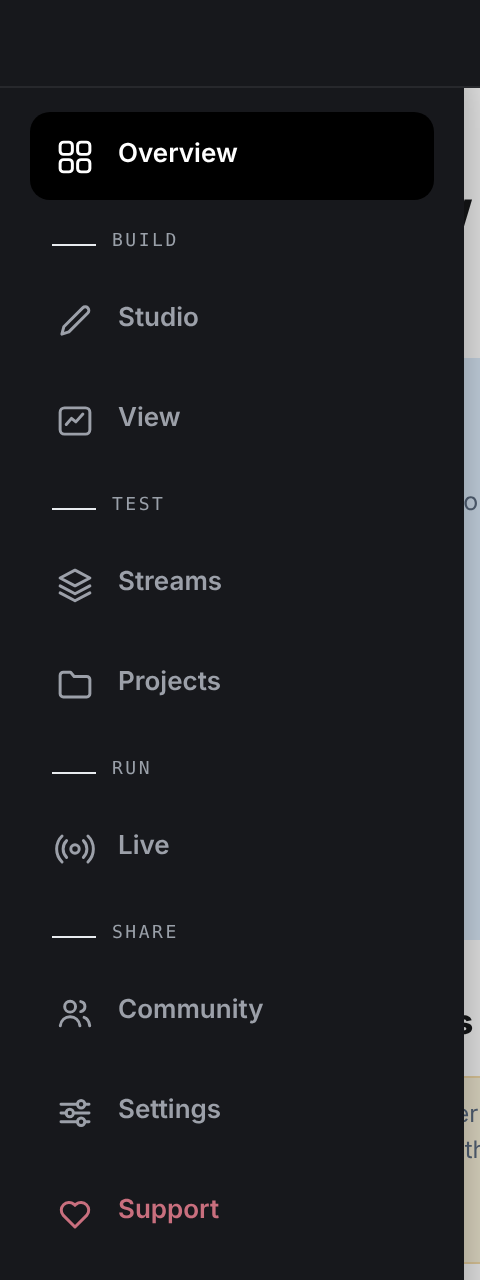
\includegraphics[width = 0.26\linewidth]
    {figure/schermate/menu.png}}}
  \caption{The menu, widened. Below \voce{Overview} the items are in four
           groups --- \voce{Build}, \voce{Test}, \voce{Run}, \voce{Share}.
           \voce{Settings} sits at the bottom.}
  \label{fig:menu}
\end{figure}

\begin{center}
\begin{tabular}{@{}L{26mm}L{18mm}L{90mm}@{}}
\toprule
\textbf{Item} & \textbf{Group} & \textbf{What it is for} \\
\midrule
\rigaTenue
\voce{Overview} & --- & The home screen: how everything is going, on one
  page. \\
\voce{Studio} & Build & Where strategies are built. \\
\rigaTenue
\voce{View} & Build & The charts, with what the strategy did drawn on
  top. \\
\voce{Streams} & Test & The results: one card per strategy. \\
\rigaTenue
\voce{Projects} & Test & Combinations of several strategies. \\
\voce{Live} & Run & The link to a real account. \\
\rigaTenue
\voce{Community} & Share & The strategy marketplace, messages, feedback and
  your own account. \\
\voce{Settings} & --- & Data, parameters, market regimes. \\
\bottomrule
\end{tabular}
\end{center}

\begin{nota}{Top right}
The magnifying glass searches the whole application; the bell shows finished
jobs and messages; the sun switches between light and dark; the last item is
the way into your account.
\end{nota}

\section{Do you need an account?}\label{sez:account-needed}

To build, test and run strategies, \textbf{no}: the application runs on your
own computer and asks for nothing.

An account is needed only for the areas that go through the network: the
\voce{Community} --- marketplace, messages, feedback, profile --- and the
subscription. If you open one of them without being signed in, the
application says so and offers to sign you in.

\section{The order in which you work}\label{sez:order}

\begin{pratica}{From nothing to the first result}
\begin{enumerate}
  \item \percorso{Settings \freccia Data}: download the data. Without data,
        every page is empty --- it is not an error, there is simply nothing
        to show.
  \item \percorso{Streams \freccia Run backtest}: choose a strategy and press
        \pulsante{Run backtest}.
  \item Wait. The job runs in the background and the bell tells you when it
        is done; meanwhile you can use the rest of the application.
  \item \voce{Streams}: the result has appeared as a card.
  \item \voce{Projects}: combine two or more results.
  \item \voce{Live}: connect a broker, when you are ready.
\end{enumerate}
\end{pratica}

% ===========================================================================
%  user/02-overview/00-chapter.tex
% ===========================================================================
\chapter{Overview}\label{cap:overview}

It is the page that opens first. It answers a single question: how is
everything going, right now.

\figuraSchermata{1.0}{figure/schermate/overview.png}
  {The home screen. Four panels: the ensemble chart, the metrics, the list of
   active streams, and the shortcut to Studio.}
  {overview}

\section{The chart at the top left}\label{sez:overview-chart}

It shows the performance of the chosen \voce{Project}: the combination of
several strategies, net of estimated costs, on the data the strategy had
\emph{not} seen while it was being built.

Until a project has been saved, an invitation to create one takes its place.
It is not an error: there is simply nothing to draw yet.

\section{Metrics OOS}\label{sez:overview-metrics}

Six numbers, and they are meant to be read together. \voce{OOS} stands for
\emph{out of sample}: computed on data the strategy did not know.

\begin{center}
\begin{tabular}{@{}L{32mm}L{106mm}@{}}
\toprule
\textbf{Metric} & \textbf{What it tells you} \\
\midrule
\rigaTenue
\voce{Sharpe ratio} & How much it earns relative to how much it swings. It is
  the number most used to compare two strategies, and the easiest to make
  look good by looking at the wrong data. \\
\voce{CAGR net} & The compound annual return, already net of estimated
  costs. \\
\rigaTenue
\voce{Max drawdown} & The largest loss from a previous peak. It is the
  question \enquote{how much would I have had to endure before recovering}. \\
\voce{Ann. volatility} & How much it swings in a year. \\
\rigaTenue
\voce{Alpha vs SPY ann.} & How much it earns \emph{beyond} the market, once
  the part explained by the market itself is removed. A strategy with a good
  return and an alpha close to zero is buying the market under other
  names. \\
\voce{Win rate} & The percentage of days in profit. On its own it says
  little: you can win nine times out of ten and still lose. \\
\bottomrule
\end{tabular}
\end{center}

\begin{perche}{Which numbers to look at first}
\voce{Max drawdown} and \voce{Alpha vs SPY}. The first because it is the
figure that decides whether a strategy can be lived with: an excellent Sharpe
with a \perc{45} drawdown is a strategy nobody holds to the end. The
second because it tells a strategy that does something apart from one that
follows the market with longer strides.
\end{perche}

\begin{attenzione}{A backtest is not a forecast}
It says how a strategy \emph{would have} behaved on past data, with
estimated costs. It does not say how it will behave. \vediCap{streams}
explains which signs tell a strategy that worked from one that got lucky.
\end{attenzione}

\section{Active streams}\label{sez:overview-list}

The list of all available results, sorted. The columns:

\begin{description}[leftmargin = 1.4em, style = nextline, itemsep = 4pt]
  \item[\voce{Sharpe}] As above.
  \item[\voce{OOS Return}] The out-of-sample return. Green above zero, red
    below.
  \item[\voce{Corr}] The correlation with the other streams. It is the column
    that matters most when combining: two highly correlated strategies, put
    together, diversify nothing --- they make the same bet twice.
  \item[\voce{Watch}] The star adds the stream to your favourites.
\end{description}

\noindent
The three menus above the list choose the period (\voce{OOS} or all of it),
the sort order and the reference project.

\section{Tutorials}\label{sez:overview-tutorials}

At the bottom right, four steps that tick themselves off as you do them:
build the first stream, validate it, combine it, put it into production. It
is the path this guide follows in the next chapters.

% ===========================================================================
%  user/03-studio/00-chapter.tex
% ===========================================================================
\chapter{Studio}\label{cap:studio}

Studio is where things are built. You get there from \voce{Studio} in the
menu, or from the \pulsante{Open Studio} button on the home screen.

\figuraSchermata{1.0}{figure/schermate/studio.png}
  {Studio. At the top the three ways of working, below them the five families
   of artifacts, in the middle the drawing board.}
  {studio}

\section{The five families}\label{sez:studio-families}

The row of tabs below the title says \emph{what} you are building. They are
five different things, and it is worth knowing which one you need before you
start.

\begin{center}
\begin{tabular}{@{}L{28mm}L{110mm}@{}}
\toprule
\textbf{Tab} & \textbf{What it is} \\
\midrule
\rigaTenue
\voce{Strategies} & A strategy: it decides what to buy and sell, and when.
  It is the thing you build most often. \\
\voce{Approaches} & An approach: it skips the whole engine and produces the
  series of gains and losses directly. It is for people who already have a
  calculation of their own and just want to bring it into the system. \\
\rigaTenue
\voce{Weight mode} & A rule for sharing capital among several strategies.
  Fourteen come already installed. \\
\voce{Overlay} & A brake: it reduces exposure when the market behaves in a
  certain way. It does not earn, it protects. \\
\rigaTenue
\voce{Metrics} & A measure to add to the ones already shown on the result
  cards. \\
\bottomrule
\end{tabular}
\end{center}

\section{The three ways to build}\label{sez:studio-modes}

At the top right you choose how to work. The result is the same --- a code
file installed in the system --- and only the road changes.

\subsection{Blueprint: with blocks}

You drag blocks from the library on the left onto the board and connect
outputs to inputs. The library is divided into categories: prices, numbers,
external data such as earnings and fundamentals.

\begin{pratica}{The quickest way to see how it works}
Press \pulsante{Load an example}: an example appears, already wired (the
crossing of two moving averages with a stop). Take it apart and put it back
together: in ten minutes you understand the mechanism without writing a
line.
\end{pratica}

\subsection{Code: by writing}

The \pulsantesec{\{ \} Code} button switches to the text editor. It is the
same artifact, seen as Python code. You can switch between the two views.

\subsection{AI agent: in words}

The \voce{AI agent} tab opens a conversation: you describe the strategy in
words and the model writes it. It needs a model installed locally; without
one, the tab says so and the other two ways keep working.

\figuraSchermata{1.0}{figure/schermate/agent.png}
  {The assistant. You describe what you want, and it writes the artifact and
   installs it.}
  {agent}

\begin{attenzione}{Read what the assistant writes}
The generated code is installed in the system and runs on your data --- and
one day, perhaps, on your account. The assistant does not know whether a
strategy makes financial sense: it knows how to write code that does what it
was asked. The \voce{Code} tab is there for this too.
\end{attenzione}

\section{Genetics}\label{sez:studio-genetics}

The \voce{Genetics} tab opens an area of its own: instead of writing one
strategy, you let many of them be born and keep those that survive. You
choose the universe of instruments and let it run.

\figuraSchermata{1.0}{figure/schermate/genetic.png}
  {The genetics section. You declare what the strategies should evolve on,
   and the rest is waiting.}
  {genetic}

\begin{nota}{It takes a long time}
It is the slowest job in the application. It starts as a background process:
you can close the page, and the bell tells you when it is finished.
\end{nota}

\section{What happens when you press \enquote{Install}}\label{sez:studio-install}

The artifact is written to a folder of the system, and from then on it
appears in the lists: a strategy among those you can run, a weighting mode
among those you can choose in a project, an overlay among those you can
switch on.

Before writing, the system checks the code: it must not read or write files,
must not open connections and must not run commands. If it contains any of
these, the installation is refused and the reason is shown.

% ===========================================================================
%  user/04-streams/00-chapter.tex
% ===========================================================================
\chapter{Streams}\label{cap:streams}

A \voce{stream} is the result of a strategy: the series of its gains and
losses over time. The \voce{Streams} page shows them all, one card each.

\figuraSchermata{1.0}{figure/schermate/streams.png}
  {The list of results. Each card carries the performance, the Sharpe ratio,
   the return and the maximum loss.}
  {streams}

\section{Running a backtest}\label{sez:run}

The \voce{Run backtest} tab, next to \voce{Streams}, lists everything that
can be run: the installed strategies and approaches, each with its own
description and a button.

\figuraSchermata{1.0}{figure/schermate/run.png}
  {What can be run. \pulsante{Run All} queues them all, one after the
   other.}
  {run}

\begin{pratica}{Running it, and then}
\begin{enumerate}
  \item Press the button of the strategy you want.
  \item The page shows the log live: you see what it is doing, line by line.
  \item You can close the page. The job carries on, and the bell at the top
        right tells you when it is done.
  \item The result appears in \voce{Streams}.
\end{enumerate}
\end{pratica}

\begin{attenzione}{One job at a time}
Backtests run in a queue, not in parallel, even if you press several
buttons. It is not a limit to work around: two calculations at the same time
would fight over the same files and produce mixed-up results.
\end{attenzione}

\section{The page of a result}\label{sez:stream-detail}

Clicking on a stream opens its page.

\figuraSchermata{1.0}{figure/schermate/stream.png}
  {The page of a stream. At the top the robustness verdict, below it the
   metrics, then the curve.}
  {stream}

\subsection{Robustness: the panel to read first}

It is the most important part of the page, and it is the one that answers
the question \enquote{did this strategy work, or was it lucky?}. The score on
the right sums up the five numbers in one.

\begin{center}
\begin{tabular}{@{}L{42mm}L{96mm}@{}}
\toprule
\textbf{Indicator} & \textbf{What it tells you} \\
\midrule
\rigaTenue
\voce{P(Sharpe > 0)} & The probability that the result is not noise. Below
  \perc{95} the strategy has proved nothing. \\
\voce{Monte Carlo p-value} & The same question asked another way: shuffling
  the data, how often would a lucky case have done just as well. The smaller,
  the better. \\
\rigaTenue
\voce{Min. track record} & How long this strategy would need to run for its
  result to be credible. A value longer than the period tested means: there
  is not enough history yet. \\
\voce{OOS Sharpe instability} & How much the Sharpe ratio changes from one
  period to the next. High means the strategy worked in some periods and not
  in others. \\
\rigaTenue
\voce{Losing OOS periods} & The percentage of periods closed at a loss. \\
\bottomrule
\end{tabular}
\end{center}

\begin{perche}{Why a \enquote{Doubtful} verdict is not an error}
It means the data are not enough to tell this strategy apart from chance.
Not that it is wrong: that it has not been proved. It is the honest answer
over a short period, and the way to change it is to have more history ---
not to change the parameters until the verdict improves, which is the most
common way of fooling yourself.
\end{perche}

\subsection{The metrics}

Ten numbers, unless you choose otherwise (see below). Besides those already
seen on the home screen (\vediCap{overview}):

\begin{description}[leftmargin = 1.4em, style = nextline, itemsep = 4pt]
  \item[\voce{Beta vs SPY}] How closely the strategy follows the market.
    Close to zero: it does something of its own. Close to one: it moves like
    the index.
  \item[\voce{Sortino}] Like the Sharpe ratio, but it counts only the
    downward swings. Rising fast is not a flaw.
  \item[\voce{Calmar}] Annual return divided by maximum loss. It answers
    \enquote{how much does it earn for each point of pain}.
  \item[\voce{Hit rate}] The percentage of periods in profit.
  \item[\voce{N obs}] How many observations. Few observations make
    everything else less reliable.
\end{description}

\subsection{Choosing the metrics}\label{sez:stream-metrics}

Every metric on the page can be hidden: the numbers, the robustness panel,
the charts, the tables, and the metrics you wrote yourself in Studio. Move
the pointer over one and a small eye appears in its corner: pressing it
hides that metric, and the message that follows has an \pulsantesec{Undo}.
To see the whole list, press \pulsantesec{Choose metrics}, at the top of
the metrics.

\figuraSchermata{1.0}{figure/schermate/stream-metrics.png}
  {\pulsantesec{Choose metrics}. Numbers, charts and tables, the default
   ones and yours, each with its tick. Next to the button, how many are
   shown.}
  {stream-metrics}

\begin{itemize}
  \item The choice holds for \emph{every} stream: you make it once.
  \item \pulsantesec{Show all}, \pulsantesec{Hide all} and
    \pulsantesec{Default} change everything at once. \voce{Default} is how
    the page looks before any choice: the default metrics and your active
    ones.
  \item A metric you create after making your choice appears by itself; you
    hide it like the others if you do not want it.
  \item Your metrics are computed only when they are shown, on the results
    of the stream and with its benchmark.
\end{itemize}

\noindent
One of your metrics can show a word instead of a value. \voce{Data not
available}: it reads data that is not in the system yet --- load it in
\percorso{Settings \freccia Data} and the metric works. \voce{Error in the
code}: the metric has to be fixed in Studio, and the word takes you there.
\voce{No results yet}: the stream has never been run.

\begin{pratica}{Adding a metric from here}
Move the pointer after the numbers, or at the very bottom of the page, below
the charts and the tables: \pulsantesec{New number metric} and
\pulsantesec{New chart metric} appear. They open the \voce{Metrics} section
of Studio with the output already chosen, a template and a free name; save,
and the metric is on the stream page (\vediSez{studio-metrics}) --- your
numbers after the default ones, your charts at the bottom, just above
\pulsantesec{New chart metric}. The pencil on one of your metrics opens it in
Studio, and Studio has a link back to the stream.
\end{pratica}

\subsection{Arranging charts and tables}\label{sez:stream-layout}

Charts and tables --- the default ones and yours --- are panels you arrange
like windows on a desktop. They stay in rows, up to three side by side.

\figuraSchermata{1.0}{figure/schermate/stream-layout.png}
  {Moving a panel. Where it was, a dashed outline; under the pointer, a small
   copy; the blue frame shows where it will land --- here the right third of
   the row, next to two other panels.}
  {stream-layout}

\begin{itemize}
  \item \textbf{Move.} Take a panel by its title bar --- the strip with its
    name --- and drag it. A blue frame shows where it will go: next to the
    panels of a row (\voce{Left half}, \voce{Middle third}\ldots), or a
    line \voce{New row} above or below a row. Let go, and the panels slide
    into place. \voce{Esc} cancels. Near the top or the bottom of the window
    the page scrolls by itself.
  \item \textbf{Make it bigger.} Pull the bottom edge of a panel down: the
    whole row grows, because panels side by side keep the same height.
    Between two panels side by side, the divider changes their widths.
    Double-click the edge or the divider: back to the normal size.
  \item \textbf{Maximize.} Double-click a panel's title: it takes the whole
    width and the height of the window. Double-click again: it goes back to
    where it was, as it was.
  \item \textbf{With the keyboard.} Among the buttons that appear on a
    panel there is one with four arrows. With the focus on it, the arrow keys
    move the panel, \voce{Shift} with the arrows change its height and width,
    \voce{Enter} maximizes it and brings it back.
\end{itemize}

\noindent
Like the choice of the metrics, the arrangement holds for every stream.
\pulsantesec{Reset layout}, in \pulsantesec{Choose metrics}, brings back
the original order: one panel per row, at the normal size. One of your
metrics that draws several charts makes one panel for each; a new chart of
yours appears at the bottom, just above \pulsantesec{New chart metric}, and
you move it where you want. In a narrow window the panels go one below the
other.

\subsection{The three buttons at the top}

\begin{itemize}
  \item \pulsante{Open the code in Studio} --- opens the artifact in the
    editor.
  \item \pulsantesec{Run backtest} --- runs the calculation again.
  \item \pulsantesec{Use in Ensemble} --- takes this stream into the project
    builder (\vediCap{projects}).
\end{itemize}

\section{View: seeing what it did}\label{sez:view}

The \voce{View} item in the menu shows prices with the strategy's trades on
top: where it went in, where it came out, and the indicators it was
watching.

\figuraSchermata{1.0}{figure/schermate/visual.png}
  {The chart view. You choose the strategy and the instrument, and overlay
   the indicators.}
  {visual}

\noindent
It is for something the numbers do not say: \emph{whether the strategy is
doing what you thought}. A curve that rises nicely can hide twenty sensible
trades and a single huge lucky one.

% ===========================================================================
%  user/05-projects/00-chapter.tex
% ===========================================================================
\chapter{Projects}\label{cap:projects}

A \voce{project} is a combination of several strategies, with the rule that
decides how much each one weighs and any brakes. It is what you put into
production: running a single strategy is rarely a good idea.

\figuraSchermata{1.0}{figure/schermate/projects.png}
  {The list of saved projects.}
  {projects}

\section{The builder, in four steps}\label{sez:builder}

It opens with \voce{Ensemble builder}, or with \pulsantesec{Use in
Ensemble} from the page of a stream. The four steps at the top always say
where you are.

\subsection{Step 1 --- Strategies}

You choose the streams to combine. You need at least two: with one there is
nothing to combine, and the \pulsante{Next} button stays off until two are
chosen.

\figuraSchermata{1.0}{figure/schermate/composizione.png}
  {Choosing the streams. Next to each one are its Sharpe ratio and return, so
   you do not have to look them up elsewhere.}
  {builder-streams}

\begin{perche}{Do not pick the best three}
The temptation is to take the three highest Sharpe ratios. It is almost
always the mistake: if the three strategies make the same bet, putting them
together reduces nothing --- you are just making it three ways. The
\voce{Corr} column on the home screen is there for this: two strategies with
low correlation, even with modest Sharpe ratios, do better together than
three good strategies that are all alike.
\end{perche}

\subsection{Step 2 --- Weighting}

How to share the capital among the chosen streams. Fourteen methods, grouped
by family.

\figuraSchermata{1.0}{figure/schermate/composizione-pesi.png}
  {The weighting methods, by family. Each one carries its line of
   explanation.}
  {builder-weights}

\begin{center}
\begin{tabular}{@{}L{36mm}L{102mm}@{}}
\toprule
\textbf{Family} & \textbf{The idea} \\
\midrule
\rigaTenue
\voce{Naive} & All the same. \voce{Equal}, an equal share each. Always worth
  trying: it is the benchmark the others are measured against. \\
\voce{Risk / covariance} & Weights by how much each one swings and how much
  they move together. Whatever swings less weighs more. \\
\rigaTenue
\voce{Robust} & As above, but without trusting the estimated correlations
  too much --- on little data they are unstable. \\
\voce{Tail-risk} & Looks at extreme losses instead of the average swing. \\
\rigaTenue
\voce{Return-aware} & Also takes into account how much each one is expected
  to earn, not only how much it risks. \\
\voce{Regime-adaptive} & Changes the weights according to the state of the
  market. \\
\bottomrule
\end{tabular}
\end{center}

\begin{pratica}{Where to start}
\voce{Equal}. Then try \voce{Min-Variance LW} or \voce{ERC} and see whether
the drawdown really falls. If a complicated method does not beat equal
weighting, equal weighting is the answer: it has one parameter fewer to get
wrong.
\end{pratica}

\subsection{Step 3 --- Overlay}

Overlays reduce exposure when something happens. Several can be switched on
together: their effects multiply, and the order in which you choose them
does not change the result.

\begin{center}
\begin{tabular}{@{}L{34mm}L{104mm}@{}}
\toprule
\textbf{Overlay} & \textbf{Reduces exposure when\ldots} \\
\midrule
\rigaTenue
\voce{Vol-Regime} & realised volatility rises. \\
\voce{Jump-Vol} & there is a sudden jump: it reacts within a day. \\
\rigaTenue
\voce{Corr-Gate} & the strategies start moving all together, that is when
  diversification disappears. \\
\voce{Regime-GMM}, \voce{Iso-Stress} & market conditions look like those of
  past periods of stress. \\
\rigaTenue
\voce{Macro-Regime} & the macroeconomic signals worsen. \\
\voce{News-Pressure} & the volume of news goes above normal. \\
\bottomrule
\end{tabular}
\end{center}

\begin{attenzione}{An overlay also takes away gains}
A brake that reduces exposure reduces everything: the losses and the gains.
It is worth looking at the two numbers together --- how much the drawdown
fell, and how much the return fell. Switching on five because \enquote{it
can't hurt} leads to a portfolio that is almost always out of the market.
\end{attenzione}

\subsection{Step 4 --- Costs}

The costs: commissions and slippage. The backtest subtracts them.

\begin{nota}{Raising the costs is the most honest check you can make}
A strategy that stays good with the costs doubled is robust. One that stops
working was earning inside the spread, and on a real account it will not
earn.
\end{nota}

\section{Saving}\label{sez:projects-save}

At the end you give it a name and save it. From then on the project appears
in the list, its performance is what the home screen draws, and --- most
importantly --- it can be chosen on the \voce{Live} page (\vediCap{live}).

% ===========================================================================
%  user/06-live/00-chapter.tex
% ===========================================================================
\chapter{Live}\label{cap:live}
% A chapter full of boxes that do not break: with the page bottom aligned,
% all the spare space ended up between two paragraphs. Here the bottom stays
% ragged; at the end of the chapter the book's alignment comes back.
\raggedbottom

This is the page where a strategy stops being an exercise. A runner always
starts in simulation: it works out the orders on the connected account and
writes them to its journal, without sending them. Real orders are switched
on runner by runner, when you decide, with an explicit confirmation. From
then on, money moves.

\figuraSchermata{1.0}{figure/schermate/live.png}
  {The Live page. At the top the status, below it the three steps to create a
   runner, on the right the summary of what is missing and the saved
   runners.}
  {live}

\section{What a runner is}\label{sez:runner}

A \voce{runner} is what runs a strategy on an account. It is made of three
parts, and they are exactly what the three steps ask for:

\begin{enumerate}
  \item \textbf{A name.} It only serves to recognise it in the list.
  \item \textbf{What it runs.} A project (with its weights and its overlays),
        or a single strategy.
  \item \textbf{Where it runs.} Which broker. For MetaTrader 5 and
        Interactive Brokers there is also the choice of orders: simulated or
        real (\vediSez{real-orders}).
\end{enumerate}

\noindent
The panel on the right shows which of the three are in place: the
\pulsante{Save runner} button stays off until all three are. Below it, a line
says what the orders will be like, already in the colour they will have on
the runner's card.

\section{The three brokers}\label{sez:brokers}

\begin{center}
\begin{tabular}{@{}L{34mm}L{104mm}@{}}
\toprule
\textbf{Broker} & \textbf{What it does} \\
\midrule
\rigaTenue
\voce{TEST} & A simulated world with synthetic data and accelerated time.
  It needs no account and no credentials. It shows whether the machinery
  works --- retraining, composition, orders --- without waiting months. It
  is always simulated. \\
\voce{MetaTrader 5} & Runs on the account the MT5 terminal installed on the
  computer is logged into: Lyra needs no credentials. At start-up it checks
  that MT5 is there; with real orders, also that the account is
  \emph{netting}, that the broker allows automated trading and that
  \voce{Algo Trading} is on. \\
\rigaTenue
\voce{Interactive Brokers} & Connects to TWS or IB Gateway with the host,
  port, client ID and account saved with \pulsantesec{Connect}. If they are
  missing, it asks for them at start-up. \\
\bottomrule
\end{tabular}
\end{center}

\begin{pratica}{The order to follow, without exceptions}
\begin{enumerate}
  \item \textbf{TEST} for a few simulated days. It shows that the machinery
        starts, that orders come out, that the journals get written.
  \item \textbf{The real broker, in simulation.} The runner reads the
        account's equity and positions and writes to the journal the orders
        it would send. You find out which instruments the broker does not
        trade and which quantities do not add up.
  \item \textbf{A demo or paper account, with real orders on.} Real orders,
        play money: you find out about trading hours, rejections and
        missing permissions.
  \item \textbf{A real account}, with a fraction of the capital.
\end{enumerate}
Skipping a step saves no time: it only means finding the same problems later,
with the money in.
\end{pratica}

\section{Simulation or real orders}\label{sez:real-orders}

Once MetaTrader 5 or Interactive Brokers is chosen, the \voce{Orders} panel
appears below the broker cards, with two positions: \voce{Simulation}, the
starting one, and \voce{Real orders}.

\figuraSchermata{1.0}{figure/schermate/live-ordini.png}
  {A runner with real orders on: the \voce{Orders} panel and the summary line
   turn red. On the right, a runner already saved in simulation.}
  {live-orders}

\begin{pratica}{Switching real orders on}
\begin{enumerate}
  \item In step~\num{3}, choose \voce{MetaTrader 5} or
        \voce{Interactive Brokers}.
  \item In the \voce{Orders} panel, press \voce{Real orders}. A window opens
        that says what changes.
  \item Read it, tick the box and press \pulsante{Enable real orders}: the
        button stays off until the box is ticked.
  \item \pulsante{Save runner}. The \voce{REAL ORDERS} label appears in red on
        the runner's card.
\end{enumerate}
For a runner that is already saved, use \voce{Switch to real orders\ldots}
on its card, with the runner stopped: the window is the same.
\end{pratica}

\figuraSchermata{0.82}{figure/schermate/live-conferma.png}
  {The confirmation of real orders. The button turns on only after the box is
   ticked.}
  {live-confirm}

\begin{attenzione}{The runner manages the whole account}
It sizes the orders on the equity of the whole account, not on a part of
it, and in the symbols it trades it closes the positions that are not among
its targets: a share bought by hand on that account, if it is in the
strategy's universe, can be sold at the next cycle. That is why the account
must be dedicated to Lyra --- one per runner, no manual trading.
\end{attenzione}

\begin{nota}{First reduce, then increase}
In every cycle the runner first sends the orders that reduce positions,
then those that increase them; a reversal (from short to long, or the other
way round) becomes two orders, the close and the open. If part of the book
cannot go out --- old data on a stock, an order still open at the broker, a
holding with no price --- or a reduction does not go through, the orders
that increase exposure wait for the next cycle. A cycle left halfway never
leaves the account more exposed than before.
\end{nota}

\noindent
The mode is always visible: on the runner's card (\voce{SIMULATION} or
\voce{REAL ORDERS}) and on every line of the journal. It can only be changed
with the runner stopped, and going back to simulation with \voce{Back to
simulation} asks for no confirmation. The \pulsante{RUN} button of a runner
with real orders is red and asks once more before starting.

\begin{nota}{The confirmation stays on record}
The runner records when real orders were confirmed, and the journal reports
it. Going back to simulation deletes the confirmation: to switch them on
again, you confirm again.
\end{nota}

\subsection{The confirmation is for one account}\label{sez:bound-account}

At the first start after the confirmation, the runner records the account it
is connected to --- on MT5 the number and server, on IBKR the number --- and
from then on it does not move. If later the MT5 terminal is logged into
another account, or the \pulsantesec{Connect} settings point to another IBKR
account, the runner does not start and the journal says which account it
expected and which one it found. If it happens while it is running, it stops
before sending anything else. The account is shown on the runner's card and
in the start window.

\begin{pratica}{Moving to another account}
\begin{enumerate}
  \item With the runner stopped, \voce{Back to simulation}.
  \item Connect the broker to the new account (the MT5 terminal, or
        \pulsantesec{Connect} for IBKR).
  \item \voce{Switch to real orders\ldots} and confirm: at the next start the
        runner binds itself to the new account.
\end{enumerate}
\end{pratica}

\begin{nota}{Accounts in another currency}
Lyra sizes the orders in dollars, on the prices of its own data. An account
in euros is fine: the equity is converted with the exchange rate the broker
gives (on MT5, the EURUSD price in the terminal). If there is no rate, real
orders do not start and the journal says so.
\end{nota}

\section{The journal}\label{sez:journal}

Every runner keeps a journal, which opens with \voce{Journal} on its card.
Everything the runner does goes into it, one line per event, with the time
and the mode in which it happened:

\begin{itemize}
  \item starts and stops, with the account it connected to: number, type
        (demo, paper or real), terminal; with real orders, also the check
        that it is the confirmed account and Lyra's orders left open,
        cancelled at start and at stop;
  \item the orders. In simulation, those it would send; if they are the same
        at the next cycle, a single line says so. With real orders, those
        sent and their outcome: filled with quantity and price, partly
        filled, still working (\emph{pending}), cancelled, rejected with the
        reason the broker gives;
  \item warnings, for example a symbol the broker does not trade, or data
        that are too old;
  \item the kill-switch events (\vediSez{kill-switch});
  \item maintenance: retraining and data updates.
\end{itemize}

\figuraSchermata{1.0}{figure/schermate/live-registro.png}
  {The journal of a runner with real orders: two orders filled, one cancelled
   because it was not filled in time, a warning.}
  {live-journal}

\noindent
The filters at the top separate orders and fills, kill-switch, warnings and
errors. While the runner is running, the journal updates by itself.

\begin{nota}{It lives on the computer}
The journal is a file in the application folder,
\file{data/runners/<id>/journal.jsonl}, one line per event; beyond
\num{5}\,MB it continues in \file{journal.1.jsonl} and so on, up to ten
files. It stays after the application is closed and even after the runner is
deleted: it is the account's logbook, and it is worth keeping.
\end{nota}

\section{The kill-switch}\label{sez:kill-switch}

Three levels, on by default, the same as in the backtest:

\begin{center}
\begin{tabular}{@{}L{30mm}L{50mm}L{58mm}@{}}
\toprule
\textbf{Level} & \textbf{When it trips} & \textbf{What it does} \\
\midrule
\rigaTenue
Strategy & An \perc{8} drawdown & Suspends it for \num{30} days, then it
  comes back by itself. \\
Asset class & A \perc{5} loss in \num{30} days & Halves its exposure for
  \num{20} days. \\
\rigaTenue
Account & A \perc{20} drawdown from the peak & Closes the positions in the
  runner's symbols and opens no others. \\
\bottomrule
\end{tabular}
\end{center}

\noindent
A suspended strategy and a halved asset class stay that way even after the
runner is restarted, until they expire.

The account level, with real orders, belongs to the \textbf{account} and not
to the runner. The drawdown is measured at the start of every cycle, before
deciding: if the fall happened between one cycle and the next, the runner
does not send another round of purchases, but closes the positions in the
symbols it trades straight away. If something stays open (market closed, a
rejection) it tries again at once, then every minute three times, then at
the normal pace; once the positions are closed, it stops by itself.

\noindent
From then on the account stays closed: after a restart, after going to
simulation and back to real orders, for any runner with real orders on that
account. Starting a runner on a closed account only serves to close the
positions left: the start window says so, the runner closes and stops. While
it is closing, not even repeated errors stop it.

\begin{pratica}{Reopening the account}
\begin{enumerate}
  \item Stop the runner.
  \item \voce{Journal} \freccia \pulsantesec{Reset kill-switch}, and confirm.
        The account reopens for every runner that uses it.
  \item At the next start the peak starts again from the account's equity.
\end{enumerate}
\end{pratica}

\begin{perche}{Why it belongs to the account, and is saved}
The kill-switch protects money, and the money is in the account. When it
belonged to the runner, a restart was enough to start again from the equity
of the moment --- after a \perc{15} drawdown the \perc{20} limit in fact
became \perc{32} --- and going to simulation and back, or using another
runner, was enough to reopen a closed account. The state lives in
\file{data/accounts/}, one file per account; if it cannot be read, real
orders do not start: a closed account must not reopen because of a damaged
file.
\end{perche}

\begin{nota}{A fall found at start-up, withdrawals and deposits}
The kill-switch looks at the account's equity and does not tell a loss from
a withdrawal. If at start-up the equity is already below the account's peak
by more than the threshold --- the fall happened with the runner stopped ---
the kill-switch trips and is recorded, but the runner sends no orders and
says how to go on. If it is a loss, start the runner again: it closes the
positions left and stops. If money was withdrawn, reset the kill-switch from
the journal instead. If the account's equity cannot be read at start-up,
real orders do not start.
\end{nota}

\begin{nota}{In simulation}
The kill-switch trips in simulation too, and the journal says what it would
have done. There it closes nothing and does not touch the account: it
belongs to the runner, and it is reset the same way.
\end{nota}

\section{When orders do not go out}\label{sez:orders-held}

When an order does not go out, or does not go as expected, the journal says
so in one line. The most common ones, what they mean and what to do:

\begin{longtable}{@{}L{46mm}L{92mm}@{}}
\toprule
\textbf{In the journal} & \textbf{What it means, and what to do} \\
\midrule\endfirsthead
\toprule
\textbf{In the journal} & \textbf{What it means, and what to do} \\
\midrule\endhead
\rigaTenue
\enquote{orders NOT sent: the data are too old}
  & The prices the runner decides on are those downloaded in
    \percorso{Settings \freccia Data}, and they do not update by themselves.
    Every symbol must reach the last closed session of its market: for US
    shares and ETFs, the New York Stock Exchange calendar, holidays
    included; for forex and crypto, one session is tolerated. A day's bar is
    expected from the following day. The orders on the symbols that are
    behind wait, and so do those that increase exposure; reductions on the
    other symbols go out. Update the data: the held orders go out at the
    first cycle with fresh data. The closes ordered by the account's
    kill-switch go out regardless. \\
\enquote{real orders cannot start on this account}
  & The account cannot receive orders from Lyra, and the line says why: on
    MT5, a \emph{hedging} account (a \emph{netting} account is needed),
    trading disabled or not allowed to expert advisors, \voce{Algo Trading}
    off, the Python API switched off in the terminal's options; on IBKR, a
    login with several accounts and no account given in
    \pulsantesec{Connect}; on both, an account in another currency with no
    rate to convert it. \\
\rigaTenue
\enquote{the real orders of this runner were confirmed for \ldots{}}
  & The broker is connected to an account different from the one the runner
    started on after the confirmation. If it is the right account, go back
    to simulation and switch real orders on again (\vediSez{bound-account}). \\
\enquote{cycle skipped, nothing sent}
  & An obstacle that appeared while the runner was on, for example
    \voce{Algo Trading} switched off or the account data not yet in sync.
    The runner skips the cycles without sending anything and resumes by
    itself when it goes away. \\
\rigaTenue
\enquote{kill-switch: this account was closed}
  & The account was closed by the kill-switch: the runner starts only to
    close the positions left, then stops (\vediSez{kill-switch}). \\
\enquote{an order is still working at the broker}
  & On that symbol there is an order still open --- Lyra's or one placed by
    hand. While it stays open, the runner does not send another: when the
    first was filled, the position would double. \\
\rigaTenue
\enquote{order(s) that add exposure not sent}
  & Part of the book did not go out (one of the lines above, or a holding
    with no price in that cycle) or a sale did not go through: in that cycle
    only the reductions go out, and the purchases are worked out again at
    the next cycle. \\
An order \emph{rejected}
  & The reason is the broker's, written in the line: permissions, market
    closed, quantity below the minimum. In TWS and IB Gateway the
    \voce{Read-Only API} option must be off, otherwise every order is
    rejected. \\
\rigaTenue
An order \emph{cancelled} on IBKR
  & It was not filled within \num{30} seconds, usually because the market
    was closed, and the runner cancelled it: left open, it would have been
    filled later while the runner was working out another one. \\
An order \emph{pending}
  & The broker accepted it but has not filled it yet (MT5), or its
    cancellation is not yet confirmed (IBKR): it can still be filled. The
    runner sends no other orders on that symbol while it stays open, and
    cancels it when it stops. \\
\rigaTenue
An order \emph{skipped}
  & The quantity is below the broker's minimum lot, and nothing went out: the
    difference is smaller than one lot. \\
\enquote{the broker is not answering}
  & Connection dropped, TWS or MetaTrader~5 closed or restarting. The runner
    sends nothing and keeps trying without giving up, with waits that grow
    up to a quarter of an hour; when the broker answers again, it says so. \\
\rigaTenue
\enquote{cycle failed (1 of 3 in a row)}
  & An error of another kind. The runner tries again within a minute; three
    errors in a row stop it, with the cause in the journal --- except when it
    is closing an account closed by the kill-switch. \\
\enquote{cannot connect to TWS/IB Gateway}
  & TWS or IB Gateway off or not logged in, API not enabled
    (\percorso{Configure \freccia API \freccia Settings}), wrong port, or
    another program is using the same client ID. \\
\bottomrule
\end{longtable}

\section{The simulator}\label{sez:simulator}

The \voce{TEST SIMULATOR} panel at the top says how long a simulated day
lasts --- in the screenshot, two seconds --- and how much time it will cover
in all. Pressing \pulsantesec{Config} changes the pace.

\begin{nota}{What speeding up time is for}
A strategy that retrains every thirty days, on a real account, retrains for
the first time in thirty days. In the simulator it happens in a minute, and
if the retraining has a problem you find out at once instead of next month.
\end{nota}

\section{Credentials}\label{sez:credentials}

The broker credentials stay \textbf{on the computer of whoever uses the
application}, in a local file. They do not go through the site, they do not
end up in any database and they do not leave the machine.

For Interactive Brokers, \pulsantesec{Connect} saves the host, the port, the
client ID and the account. Port and client ID must be numbers, and the window
says so at once. The usual ports are \num{7497} for TWS in paper and
\num{7496} for real, \num{4002} and \num{4001} for IB Gateway. The account
must be given if the login manages more than one.

\begin{attenzione}{Two consequences}
The first: nobody can recover them for you: if they are lost, you set them
up again with the broker. The second, more important: whoever has access to
that computer has access to the account. The application is meant to run on
a personal machine, not on a server others can reach.
\end{attenzione}

\section{Starting and stopping}\label{sez:start-stop}

Once saved, the runner appears in the list at the bottom right, with the
commands to start and stop it. The two counters at the top ---
\voce{RUNNING} and \voce{STOPPED} --- say how many are in each state.

\figuraSchermata{1.0}{figure/schermate/live-runner.png}
  {Two runners on the same model: one stopped in simulation, one running
   with real orders.}
  {live-runner}

\noindent
The first cycle starts at once. The following ones follow the shortest bar
among those the runner watches, a quarter of a bar at a time: for daily
strategies, one cycle every six hours. Asking the broker more often would
produce identical cycles.

\noindent
With real orders, \pulsante{RUN} asks for confirmation once more and says
which account the orders will go to; if the account was closed by the
kill-switch, it says that starting will only serve to close positions.

\begin{nota}{Stopping: no new orders}
Once \pulsante{Stop} is pressed, the orders of the current cycle not yet sent
do not go out any more; those already sent reach their outcome, which goes
into the journal. With real orders, Lyra's orders still open at the broker
are cancelled: none of them is filled later without the runner watching.
\end{nota}

\begin{attenzione}{One broker per runner}
Two runners on the same account fight over the positions: the first opens,
the second sees a position it does not expect and closes it. The page says
so in step~\num{3}, and does not let a second runner start on the same
broker while the first is running.
\end{attenzione}

\flushbottom

% ===========================================================================
%  user/07-community/00-chapter.tex
% ===========================================================================
\chapter{Community}\label{cap:community}

It is the area where users meet, and the only one in the application that
needs an account. In the menu it sits under \voce{Share}; the page has four
tabs:

\begin{center}
\begin{tabular}{@{}L{34mm}L{104mm}@{}}
\toprule
\textbf{Tab} & \textbf{What it is for} \\
\midrule
\rigaTenue
\voce{Marketplace} & Buying and selling strategies, approaches, overlays and
  weighting methods. It is the subject of this chapter. \\
\voce{Messages} & Conversations with other users, for example with the
  author of a strategy. \\
\rigaTenue
\voce{Feedback} & The reports and suggestions sent to the Lyra team. \\
\voce{My account} & Profile, security and subscription
  (\vediCap{account}). \\
\bottomrule
\end{tabular}
\end{center}

\figuraSchermata{1.0}{figure/schermate/marketplace.png}
  {The \voce{Community} without an account. The rest of the application keeps
   working: the page says so.}
  {community-signed-out}

\section{Why an account is needed here and not elsewhere}\label{sez:why-account}

Because here there is someone on the other side. Building and testing
strategies happens entirely on your own computer, and asking for an account
to do it would make no sense. Buying, selling and granting a licence require
the system to know who is who.

\section{Buying}\label{sez:buy}

\begin{pratica}{From the storefront to the system}
\begin{enumerate}
  \item Open the artifact's page: description, metrics declared by the
        seller, comments, sometimes a video.
  \item \pulsante{Buy} --- if it is free, access is immediate; if it is paid,
        the payment flow opens.
  \item Once the payment is done you go back to the application. If access
        does not show as active yet, \textbf{it is not an error}: the
        confirmation arrives a moment later. The page says so and asks you to
        wait.
  \item \pulsante{Install} --- the artifact is written to the system, and
        from then on it appears in the lists like all the others.
\end{enumerate}
\end{pratica}

\begin{nota}{Before installing, the conflicts}
If something with the same name already exists in the system, the
application says so \emph{before} writing. It is worth reading: an
installation that overwrites a strategy you were working on is lost work.
\end{nota}

\subsection{If a purchase does not show up}

There is a command for exactly this, on the artifact's page, that explains
why it does not show as purchased. It tells apart two things that at first
sight look the same: \enquote{you did not buy it} and \enquote{I could not
ask}. They are opposites, and the second is solved by trying again.

If the payment went through but access does not open, there is a
reconciliation command: it checks the payment again with the provider and,
only if it shows as collected, completes the operation.

\section{Selling}\label{sez:sell}

To publish you need two things, in this order:

\begin{enumerate}
  \item \textbf{The marketplace must be open.} During the beta it is closed:
        nobody uploads anything. Items already in the storefront stay
        visible.
  \item \textbf{A paid plan.} With the marketplace open, any paid plan will
        do, from Pro up (\vediCap{account}). On Free you can browse, download
        and buy, but not sell.
\end{enumerate}

\begin{perche}{Why a subscription even to publish for free}
It is not about the money. Whoever publishes puts their name next to a
strategy that others will run with their own money: a filter at the entrance
is worth more than any check after the fact. Someone without a subscription
remains a full user --- they browse, download, buy and use. They just cannot
put things in the storefront.
\end{perche}

\noindent
A published artifact goes online at once: there is no approval queue. The
description and the video can be corrected later; the bundle of files
cannot.

\section{If an artifact does not perform as declared}\label{sez:dispute}

You open a dispute from the artifact's page. It is not a discussion: the
system runs two automatic checks.

\begin{center}
\begin{tabular}{@{}L{44mm}L{94mm}@{}}
\toprule
\textbf{Check} & \textbf{What it compares} \\
\midrule
\rigaTenue
\voce{Integrity} & The installed files with those sold, one by one. \\
\voce{Performance} & The metrics declared by the seller with those obtained
  by running the calculation again on your own system. \\
\bottomrule
\end{tabular}
\end{center}

\noindent
The case is a conversation between buyer, seller and the administration,
with the results of the two checks attached. It can be withdrawn at any
time.

\begin{nota}{Two different results do not mean a deception}
A strategy can perform differently because the data are different: a
different universe of instruments, a different period, different costs. The
check is there to establish \emph{by how much} they differ, which is the
starting point of any sensible discussion.
\end{nota}

% ===========================================================================
%  user/08-settings/00-chapter.tex
% ===========================================================================
\chapter{Settings and data}\label{cap:settings}

The \voce{Settings} item gathers three tabs: \voce{Config}, \voce{Data} and
\voce{Market rules}. They are the three places where you tell the system
what to work with, and within which limits.

\section{Data: bringing in the prices}\label{sez:data}

Without data, every page of the application is empty. It is the first thing
to do after installing.

\figuraSchermata{1.0}{figure/schermate/data.png}
  {The Data page. On the left the automatic download, on the right the manual
   upload, below them the categories.}
  {data}

\subsection{Downloading}

You choose three things and press \pulsante{Download}:

\begin{description}[leftmargin = 1.4em, style = nextline, itemsep = 4pt]
  \item[\campo{Provider}] Where to get them from. Some need a personal key,
    which you set up from the site.
  \item[\campo{Timeframe}] The time step. The same instrument can exist at
    several steps: daily data and five-minute data live in different folders
    and do not get in each other's way.
  \item[\campo{Category}] What kind of data it is.
\end{description}

\noindent
The job goes into the queue and the bell tells you when it is done. Below the
fields, a line says what is already there: how many files, how much space, up
to when they go.

\subsection{Uploading your own file}

The \voce{Your data} panel accepts CSV, Parquet and XLSX files dragged onto
it. The system recognises by itself columns written in capitals, dates given
as an index or as a column, and prefixes such as \campo{adj\_}. The
\voce{Expected format} panel shows what it expects.

\subsection{The categories}

Each category is a folder, and they come in two types.

\begin{center}
\begin{tabular}{@{}L{22mm}L{116mm}@{}}
\toprule
\textbf{Type} & \textbf{It means} \\
\midrule
\rigaTenue
\voce{1:1} & One file per instrument, named after the instrument. The link
  is automatic, and the application can say how many instruments are covered
  and how many are not. \\
\voce{1:N} & Files shared by several instruments: sectors, macroeconomic
  series, currencies. Here there is no coverage to compute, and the strategy
  has to declare which file to use. \\
\bottomrule
\end{tabular}
\end{center}

\begin{nota}{\enquote{0 / 15 assets covered} is not a fault}
It means the category exists but has no data yet for any instrument. It
fills up by downloading, or by dragging files into it.
\end{nota}

\section{Config: the limits}\label{sez:config}

These are the parameters that apply to every calculation.

\figuraSchermata{1.0}{figure/schermate/config.png}
  {The parameters. Each field carries its unit below it, because the
   difference between \num{0.12} and \num{12} is a factor of a hundred.}
  {config}

\begin{center}
\begin{tabular}{@{}L{44mm}L{94mm}@{}}
\toprule
\textbf{Field} & \textbf{What it limits} \\
\midrule
\multicolumn{2}{@{}l}{\textit{\small Portfolio \& allocator}}\\[2pt]
\rigaTenue
\voce{Initial capital} & The capital the calculations start from. \\
\voce{Annual target volatility} & How much you accept the portfolio swinging
  in a year. It is the main risk dial. \\
\rigaTenue
\voce{Max weight per position} & The most a single instrument can weigh. \\
\voce{Max gross per asset class} & The most a whole class can weigh ---
  shares, bonds, currencies. It guards against diversification that is only
  apparent: four bonds all going the same way are a single position. \\
\rigaTenue
\voce{Max gross leverage} & The total exposure. \num{1.0} means no
  leverage. \\

\addlinespace
\multicolumn{2}{@{}l}{\textit{\small Ensemble}}\\[2pt]
\rigaTenue
\voce{Target volatility} & The volatility every stream is brought to
  \emph{before} being weighted. \\
\voce{Regime window}, \voce{thresholds} & How the state of the market is
  assessed for the modulation. \\
\bottomrule
\end{tabular}
\end{center}

\begin{attenzione}{\voce{Target volatility} also acts on the real account}
It is not a display setting. The same factor that normalises the streams in
the backtest multiplies the positions the runner opens on a real account.
Changing it changes how much you really risk, not just what you see on the
chart.
\end{attenzione}

\noindent
Further down, \voce{Asset categories} lets you add categories of
instruments: once created, a strategy can declare them and restrict itself to
them.

\section{Market rules: the regimes}\label{sez:regimes}

A \voce{regime} is the state of the market, with three values: \voce{bull},
\voce{neutral}, \voce{bear}. Strategies can declare that they weigh things
differently according to the state.

\figuraSchermata{1.0}{figure/schermate/regime.png}
  {The configured markets. Below them, the history of the states: green bull,
   grey neutral, red bear.}
  {regime}

\subsection{How to read the page}

Each panel at the top is a \emph{market} --- a set of instruments that share
the same way of measuring the regime:

\begin{description}[leftmargin = 1.4em, style = nextline, itemsep = 4pt]
  \item[\voce{RULE}] The rule used to compute the state.
  \item[\voce{DRIVER}] The series that drives the decision --- for shares,
    SPY; for forex, the dollar.
  \item[\voce{SYMBOLS}] How many name patterns fall into this market.
  \item[The coloured bar] How much time was spent in each state.
\end{description}

\begin{attenzione}{\enquote{No driver available}}
The panel of a market that cannot find its driving series says so with a
warning, like the \voce{crypto} market in the screenshot. That market
\textbf{modulates nothing}: it is not an error that blocks anything, but the
strategies on those instruments behave as if the regime were always neutral.
The fix is to download the missing series from the \voce{Data} page.
\end{attenzione}

\subsection{The chart}

It shows the driving series with the background coloured by state. Below it,
the counts: how many observations, how many times the state changed, and the
percentage of time spent in each.

\begin{nota}{Few changes of state is a good thing}
A regime must be a \emph{state}, not a reaction. Twenty-five transitions in
five years mean the rule tells different periods apart; two hundred would
mean it is chasing noise, and a strategy that changes weight every week pays
costs without taking a position.
\end{nota}

% ===========================================================================
%  user/09-account/00-chapter.tex
% ===========================================================================
\chapter{Account and subscription}\label{cap:account}

\section{What the account is for}\label{sez:account-for}

Four things, and nothing else: entering the marketplace and receiving
messages --- both in the \voce{Community} --- having a public profile, and
taking out a subscription. The rest of the application works without one.

\figuraSchermata{0.86}{figure/schermate/subscription.png}
  {Pages that need an account say so and offer to sign you in, instead of
   disappearing from the menu.}
  {signed-out}

\section{Signing in for the first time}\label{sez:first-sign-in}

\begin{pratica}{During the beta}
During the beta, access is reserved for people who signed up on the site.
The first sign-in is not a registration: it is a password reset.

\begin{enumerate}
  \item On the sign-in page, choose \voce{Forgotten your password?}.
  \item Enter the address you used to sign up for the beta.
  \item A message arrives with a code; use it to set a new password.
  \item From then on you sign in normally.
\end{enumerate}

An address that is not among the sign-ups is refused, both at sign-in and at
registration.
\end{pratica}

\noindent
You can also sign in with Google (\voce{Continue with Google}): the sign-in
opens in the system browser and the application picks up the result.

\section{The profile}\label{sez:profile}

\voce{Profile}, in the account menu at the top right, gathers the account on
one page. \pulsante{Sign out} is at the top right of the page.

\figuraSchermata{1.0}{figure/schermate/profile.png}
  {The top of the profile: the plan, two-step verification, the payout account
   and the published artifacts at a glance; below, the account details,
   marketplace publishing and earnings.}
  {profile}

\begin{description}[leftmargin = 1.4em, style = nextline, itemsep = 4pt]
  \item[\voce{Account details}] Display name and bio --- what others see next
    to a published artifact --- changed with \pulsantesec{Edit profile}.
  \item[\voce{Marketplace publishing}] Whether you can sell, with links to
    your purchases and your listings, and to \voce{My subscription}.
  \item[\voce{Marketplace earnings}] The payout account that receives what
    you sell. Selling for a price needs one, and linking it needs two-step
    verification first.
  \item[\voce{Security}] The password, the email address and two-step
    verification. They are not stored by the application: they live on the
    site, and the application only passes them on.
  \item[\voce{Preferences}, \voce{Brokers and data keys}] The theme and the
    notifications; the broker connections and the data keys, which stay on
    this computer.
  \item[\voce{Send us feedback}] A report or a suggestion for the Lyra
    team.
\end{description}

\section{The plans}\label{sez:plans}

The plans are the same as on the Pricing page of the site. Free is the whole
application; you pay for privacy, data and a higher share of what your
strategies earn --- not for using the application. They are on the
\voce{My subscription} page, in the account menu at the top right.

\begin{center}
\begin{tabular}{@{}L{22mm}L{30mm}L{86mm}@{}}
\toprule
\textbf{Plan} & \textbf{Price} & \textbf{What it adds} \\
\midrule
\rigaTenue
\voce{Free} & \eur{0}, forever & The whole application: building and
  backtesting locally with your data, the local AI copilot, out-of-sample
  validation, live runners and kill-switch. On the marketplace: browse,
  download, buy. Share of earnings \perc{0}: an allocated strategy enters the
  track record. \\
\voce{Pro} & \eur{49} a month or \eur{490} a year & Full privacy for code
  and metrics; selling on the marketplace and buying at $-$\perc{10}; the
  institutional-data sandbox (from 2030); \perc{10} of what your allocated
  strategies earn. \\
\rigaTenue
\voce{Professional} & \eur{149} a month or \eur{1,490} a year & Raw history
  on your machine (from 2030) with $-$\perc{10} on data vendors; marketplace
  $-$\perc{20}; sandbox on more markets; \perc{30} of earnings. It is the
  recommended plan. \\
\voce{Quant} & from \eur{200} a month or \eur{2,000} a year, plus data &
  Exchange-licensed real-time (from 2032), in per-market packages; extended
  sandbox; \perc{30} of earnings. \\
\rigaTenue
\voce{Desk} & \eur{8,000} a year & Five seats, installation on your servers,
  compliance export, white-label and SLA; \perc{30} of earnings, per seat, by
  contract. Sold by contract, after a demo. \\
\bottomrule
\end{tabular}
\end{center}

\figuraSchermata{1.0}{figure/schermate/subscription-plans.png}
  {The plans on \voce{My subscription}: price, share of earnings and what
   each plan adds. \voce{Show the detailed comparison} opens the table with
   every feature, plan by plan.}
  {subscription-plans}

\begin{nota}{The features with a year}
Some features arrive with a later release: the sandbox and the raw history
in 2030, real-time in 2032. The cards and the comparison table show the year
next to them.
\end{nota}

\begin{nota}{During the beta}
The paid plans open after the beta. Until then Free is the whole
application, nothing can be bought or sold on the marketplace, nothing is
charged, and the plan buttons say \voce{On sale after the beta}. A Desk demo
can be requested already.
\end{nota}

\begin{nota}{The share of earnings}
It is the part of what a strategy earns, once it is allocated to capital,
that goes to its author: \perc{10} with Pro, \perc{30} with Professional,
Quant and Desk, set by contract. On Free an allocated strategy enters the
track record without a share. Every submission is opt-in, strategy by
strategy and under a contract: nothing is submitted without your consent.
The site describes the steps, from the protocol to the live track record.
\end{nota}

\subsection{The two-month trial}

Pro, Professional and Quant start with a two-month trial, one per account.

\begin{pratica}{Starting the trial}
\begin{enumerate}
  \item On the plan's card, press \pulsante{Start 2-month trial}; the hint
        below the button says until when nothing is charged.
  \item The window shows \voce{Charged today} at \eur{0}, the day the trial
        ends and the price that applies afterwards. Choose monthly or yearly
        there, then press \pulsante{Start the trial}.
  \item The Stripe page opens: Stripe asks for your card but charges
        nothing. The page updates by itself and shows \voce{Trial until} and
        the date.
  \item On that date the first payment is taken. Cancel before, and nothing
        is ever charged.
\end{enumerate}
\end{pratica}

\noindent
Changing plan during the trial costs nothing, and the trial keeps its end
date. An account that has already had a trial, or a paid plan, pays from the
first day: the button then says \pulsante{Choose} followed by the plan's
name.

\subsection{Desk}

Desk is not bought with a card: it starts with a demo on your firm's own
strategies, and a contract. \pulsantesec{Request a demo} on the Desk card
opens a short form --- the firm, how many people would use the platform, a
message --- and the request reaches the Lyra team, who reply by email and in
\voce{Messages}.

\subsection{Monthly or yearly}

Both. Yearly costs ten monthly payments: two months are free. Desk is yearly
only. You choose when you subscribe and switch whenever you like, from the
button next to your plan: Stripe works out the adjustment for the period
already paid.

\subsection{Changing plan}

\pulsantesec{Upgrade} and \pulsantesec{Downgrade} on the cards change the plan
at once: Stripe credits what you have already paid for the current period and
charges the difference to the card on file. Before you confirm, the window
lists what you gain or what you lose.

\subsection{Cancelling, card, invoices}

From \pulsante{Manage in Stripe} on \voce{My subscription}. The billing
portal hosted by Stripe opens: there you cancel the subscription, change the
payment method and download the invoices. The card never reaches the
application.

\begin{nota}{Cancelling takes nothing you already have}
The plan stays active until the end of the period you paid for. A purchased
artifact stays purchased and installed, and strategies, code and data stay on
your computer: you go back to Free, which is still the complete application.
What stops is selling on the marketplace and the benefits of the plan.
\end{nota}

\section{When something does not add up}\label{sez:account-problems}

\begin{center}
\begin{tabular}{@{}L{50mm}L{88mm}@{}}
\toprule
\textbf{Symptom} & \textbf{What to do} \\
\midrule
\rigaTenue
\enquote{You cannot sell} but you have a subscription
  & Close and reopen the application: the link with the site is made at
    start-up. \\
The marketplace is empty
  & Same reason. If it persists, sign out and sign back in. \\
\rigaTenue
I paid and I cannot see the artifact
  & Wait a few seconds and reload. If it stays like that, use the command
    that explains why it does not show as purchased, on the artifact's page
    (\vediCap{community}). \\
The trial is not offered
  & The trial is one per account: an account that has already had one, or a
    paid plan, pays from the first day. \\
\rigaTenue
A page says it does not know, instead of showing a number
  & Not a fault: the application could not ask the site, and says so instead
    of making up an answer. Try again later. \\
\bottomrule
\end{tabular}
\end{center}


\end{document}
